%%%%%%%%%%%%%%%%%%%%%%%%%%%%%%%%%%%%
\chapter{Results and Discussions}
\label{chap:Results}
%%%%%%%%%%%%%%%%%%%%%%%%%%%%%%%%%%%%

\section{Experimental Settings}
\label{experimental_settings} 
The settings for all experiments were conducted using test trains split defined by \cite{Talebi2018}, and data augmentation outlined in chapter \ref{chap:Methodology}, with input of raw images resized to $3 \times 224 \times 224$. To enable effective side-by-side comparison with baseline, state of the art pre-processing steps are kept the same. We also used transfer learning from the same source dataset, ImageNet1k. Transformers and CNNS are, however, inherently different - for example, learning rate alongside approaches such as warming-up\cite{Zhang2021} are necessary for transformers to converge, therefore some aspects - such as learning rate - change during training of baseline and transformer models. 

%%%%%%%%%%%%%%%%
% FLOW CHART %%%
%%%%%%%%%%%%%%%%

\subsection{ResNets and ConViTS}


We conduct experiments to obtain baselines using ResNets $\in\{18,50,152\}$ and ConViT models $\in\{tiny,small,base$\}$ $, which are pre-trained on ImageNet-1k, and added an additional, fully connected layer to correspond to binary classes. Hyper parameter selection is a crucial part of tuning and adapting models to the target domain. 


%%%%batch_size=50
%color_jitter=0.4, 
%cooldown_epochs=10,
%lr=0.0005, 
%local_up_to_layer=10, 
%locality_strength=4.0, 
%lr_noise_pct=0.67, 
%opt='adamw',
%opt_eps=1e-08, 
%sched='cosine', 
%warmup_epochs=5, 
%warmup_lr=1e-06, 
%weight_decay=0.05, 


\begin{table}[ht!]
\small
\centering
\caption{Hyper Params}
\begin{tabular}{c?ccc}
\toprule
Hyper Param &  \multicolumn{1}{c}{ResNet innitial} & \multicolumn{1}{c}{ConViT} & Equal Conditions\\
\midrule
Learning Rate     &  0.0001        & 0.0005          & 0.0003         \\
Colour Jitter     &  0.5           & 0.5             & 0.5            \\
Optimiser         &  $Adam$        &  $AdamW$        & $AdamW$        \\
Batch size        & 50-250         & 10-200          & 10-200         \\
Loss Function     & $cross entropy$& $cross entropy$ & $cross entropy$\\
Cool down epoch   & -              & 5               & 0              \\
Scheduler         & $StepLR$       & $cosine$        & $cosine$       \\
Opt. $\epsilon$    & -             & 1e-08           &                \\
Local up to layer & -              & 10              & -              \\ 
Locality strength & -              & 4.0             & -              \\ 
lr noise pct.     & -              & 0.67            & 0              \\ 
Warm up epochs    & -              & 5               & 3              \\
Warm up lr        & -              & 1e-06           & 1e-06          \\
\bottomrule
\end{tabular}
\end{table}

\subsection{Optimiser and Scheduler}
These differ slightly between ConViT and baseline models. 

\begin{description}
\item[For ConViTs] We use AdamW with a Cosine\footnote{\href{https://github.com/rwightman/pytorch-image-models/blob/master/timm/scheduler/cosine_lr.py}{https://github.com/rwightman/pytorch-image-models/blob/master/timm/scheduler/cosine\_lr.py}}  learning rate Scheduler;
\item[for ResNets] we use Adam and AdamW with Stepped learning rate scheduler and cosine scheduler;
\item[for ViT and CvT] we use Adam with Cosine learning rate scheduler;
\end{description}

We use an Adam optimiser\cite{Kingma2015} as gradient base optimisation for simplicity of implementation and computational efficiency. We use a Cosine Scheduler by \cite{DAscoli2021} for ConViTs, as there is clearly a trade-off in keeping domain parameters the same. Both schedulers are a form of simulated annealing, which allowed for a change in learning rate over time - mitigating against the challenges of gradient based approaches, such as saddle points. 

We train networks in separate code environments\footnote{\href{https://github.com/facebookresearch/convit}{https://github.com/facebookresearch/convit}}, using code supplied by \cite{DAscoli2021} for ConViTs and CvT. We train all models under equal conditions, in the same code environment, with identical training and data augmentation pipelines. Various aspects, such as data augmentation, are inherent features of training pipeline.

\subsection{Loss Function Vs Data Sampler}

Loss function is necessary to minimise the difference between GT labels, and where minimisation of loss or error between GT and predicted result is required.  While formative experiments were conducted with focal loss, we adopt a cross entropy loss function. While \cite{Lin2020} have shown that focal loss, combined with cross entropy, have been shown to be effective techniques in addressing class imbalance. 

We use cross entropy with a sampler, where random sampling from the minority class with a weighted probability is used to address this. This is effective, as it allows repeated augmentation of the minority class during training. Further, this is the technique used in code for training on ImageNet-1k by \cite{Touvron2020a, DAscoli2021}, and therefore provides methodological consistency across baseline and vision transformer models .\lstinline[language=Python]{torch.utils.data.sampler.WeightedRandomSampler}

Where samples are computed for every batch given by:
\begin{equation}
    Sc = \frac{\sum_{i=1}^{Bn}}{\sum_{i=1}^{Cn}}
    \label{eq:class weights} 
\end{equation}

Where $Sc$ s sample ratio $Bn$ is the number of batch samples, and $Cn$ n is the class count of each batch.

\subsection{Software and Hardware}
The experiments were conducted using a single Nvidia Tesla P100 12Gb GPU, with CUDA 11.2. The software used for training was PyTorch open source framework, with data ammunition using both Torchvision's native fictions alongside Albumentations\cite{Buslaev2020a}. ConViT models were built using timm\footnote{\href{https://github.com/rwightman/pytorch-image-models/tree/master/timm}{https://github.com/rwightman/pytorch-image-models/tree/master/timm}}. All software is implemented using Python 3.7.

\begin{table}[]
    \centering
    \begin{tabular}{c?cc}
    \toprule
     Software & Version & Purpose \\
     \midrule 
     torch &   1.7.0 & Training ConViTs\\
     timm & 0.3.2 & Building ConViTs\\
     albumentations & 0.4.6 & Data augmentation\\
     torchvision & 0.8.1 & Pre-trained models\\
     \bottomrule
    \end{tabular}
    \caption{Software}
    \label{tab:software}
\end{table}

\section{Quantitative Results}
\label{Quantitative Results} 
\subsection{Training}
\subsubsection{ResNets}
Training ResNets for 10 epochs shows differences in overall accuracy. These are shown in figure \ref{fig:resnet_train}. In training and validation accuracy, loss, and balanced accuracy, all layers were unfrozen to allow pre-trained models to be fully adapted during training.

\begin{figure}[ht!]
    \begin{center}
    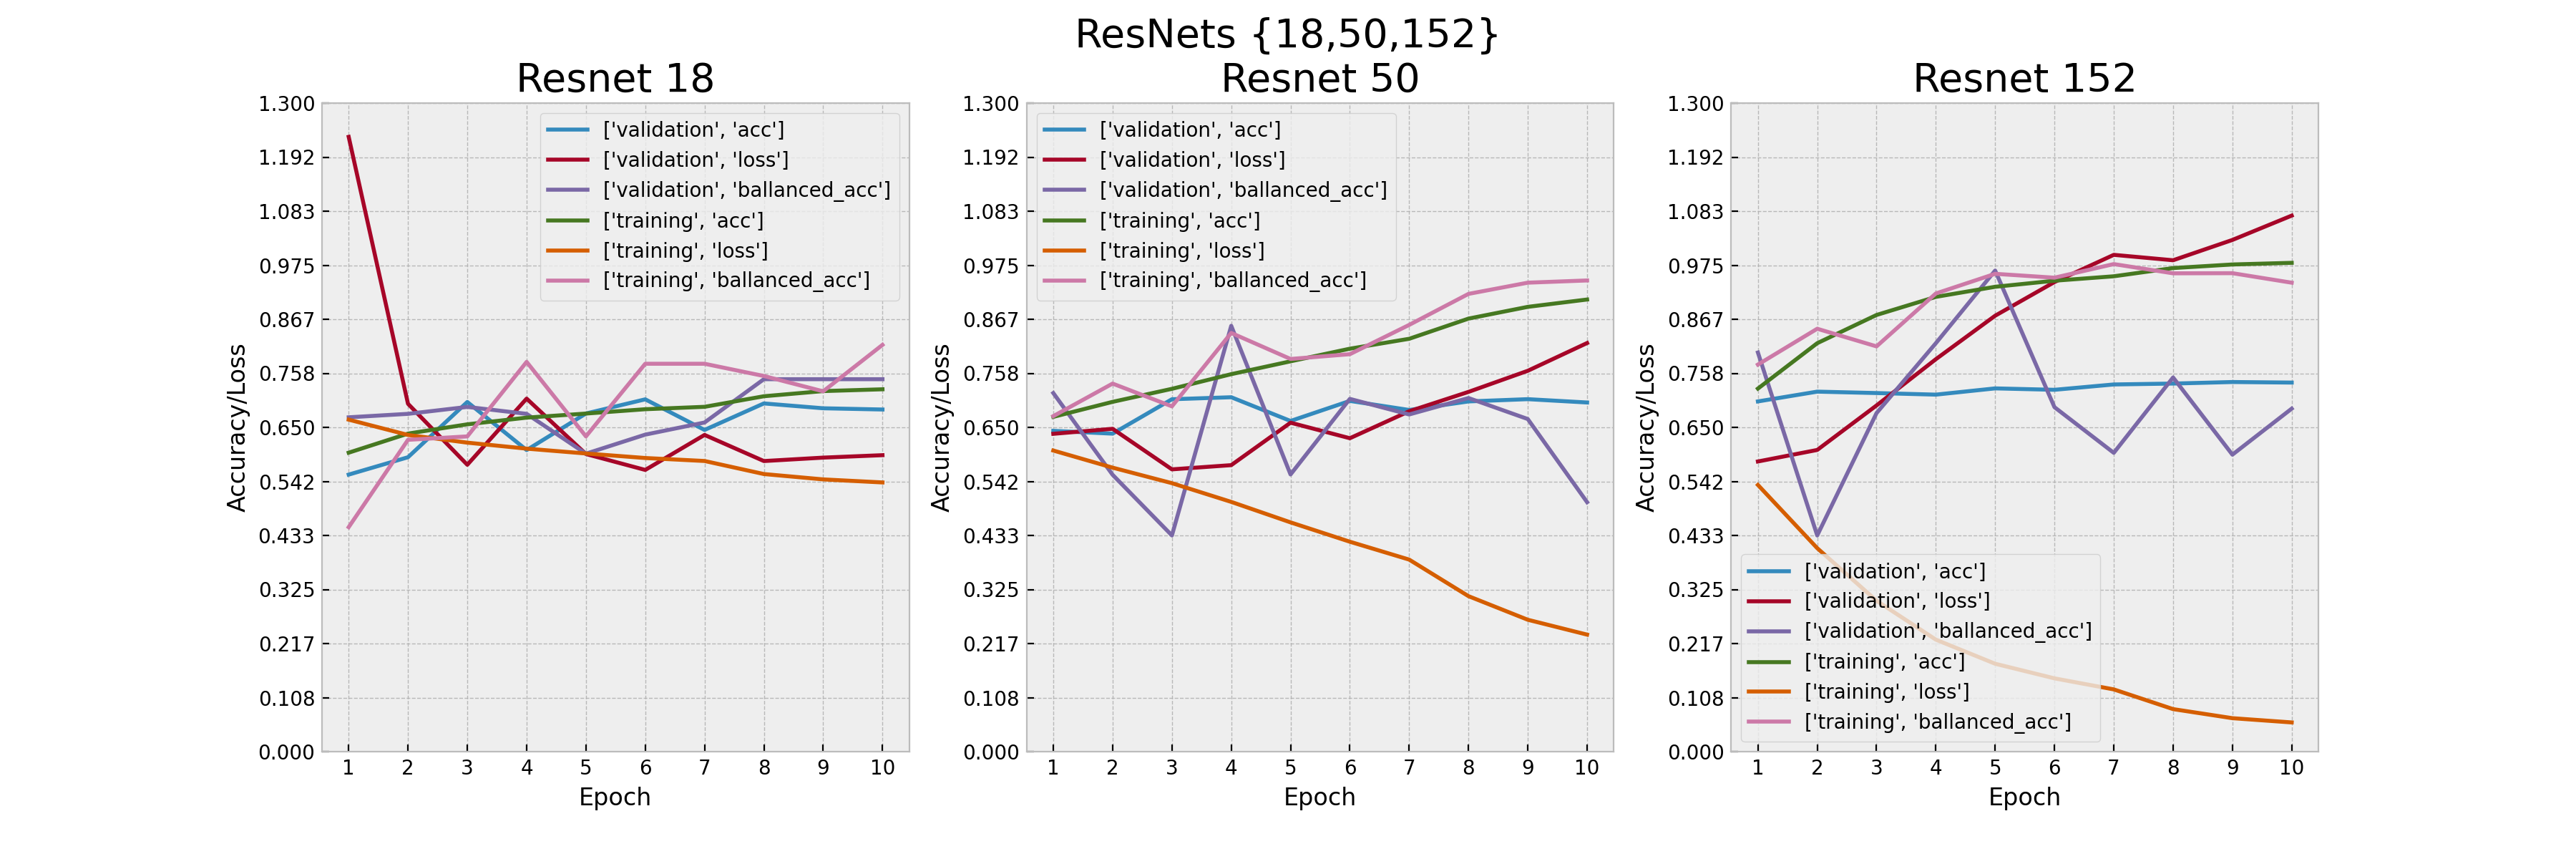
\includegraphics[height=0.3\textwidth]{figures/results_and_discussion/resnets.png}
    \caption{ Side by Side Comparison of ResNets}
    \label{fig:resnet_train}
    \end{center}
\end{figure}

Note that only ResNet18 converges after pre-training, which importantly shows that ResNet18's depth may not have enough trainable parameters or be deep enough to produce the best results. Further, note that after convergence there is very little improvement of training or validation accuracy. 

Balanced accuracy shows more instability, indicating that accuracy in itself may be `masking' model fitting. However, both appear similar where equal numbers of positive and negative classes are sampled in each training batch. 

ResNet152 continues improvement in accuracy and balanced accuracy (there is also less difference). This indicates that when a model has sufficiently trainable parameters and is deep enough that there is a high degree of similarity to features that are trained on ImageNet21k. 

\begin{table}[ht!]
\centering
\small 
\begin{tabular}{lcccccccc}
\toprule
{} & \multicolumn{2}{c}{Resnet 18} & {}& \multicolumn{2}{c}{Resnet 50} & {}& \multicolumn{2}{c}{Resnet 152} \\ 
 \midrule
{} & Validation & Training &{} & Validation & Training &{} & Validation & Training \\
\cline{2-3} \cline{5-6} \cline{8-9}
Accuracy &      0.706 &    0.726 & &      0.710 &    0.906 & &      0.741 &    0.980 \\
Balanced Acc &      0.747 &    0.815 & &      0.854 &    0.944 & &    0.964 &    0.977 \\
\bottomrule
\end{tabular}
\caption{ArgMax Resnet Training Metrics}
\label{tab:resnet train}
\end{table}


Table \ref{tab:resnet train} shows the differences in training accuracy and balanced accuracy - there is a clear improvement in increasing model size over the same number of epochs. 

\subsubsection{CvT and ConVits}

We train both CvT\cite{Wu2021} and ConViTs to enable side by side comparison. Results from training CvT\cite{Wu2021} show that a model will converge after 5 of epochs (see figure \ref{fig:CvT} right), however, the model quickly plateaus. This can be seen in figure \ref{fig:CvT} left.
\begin{figure}[htp!]
    \centering
    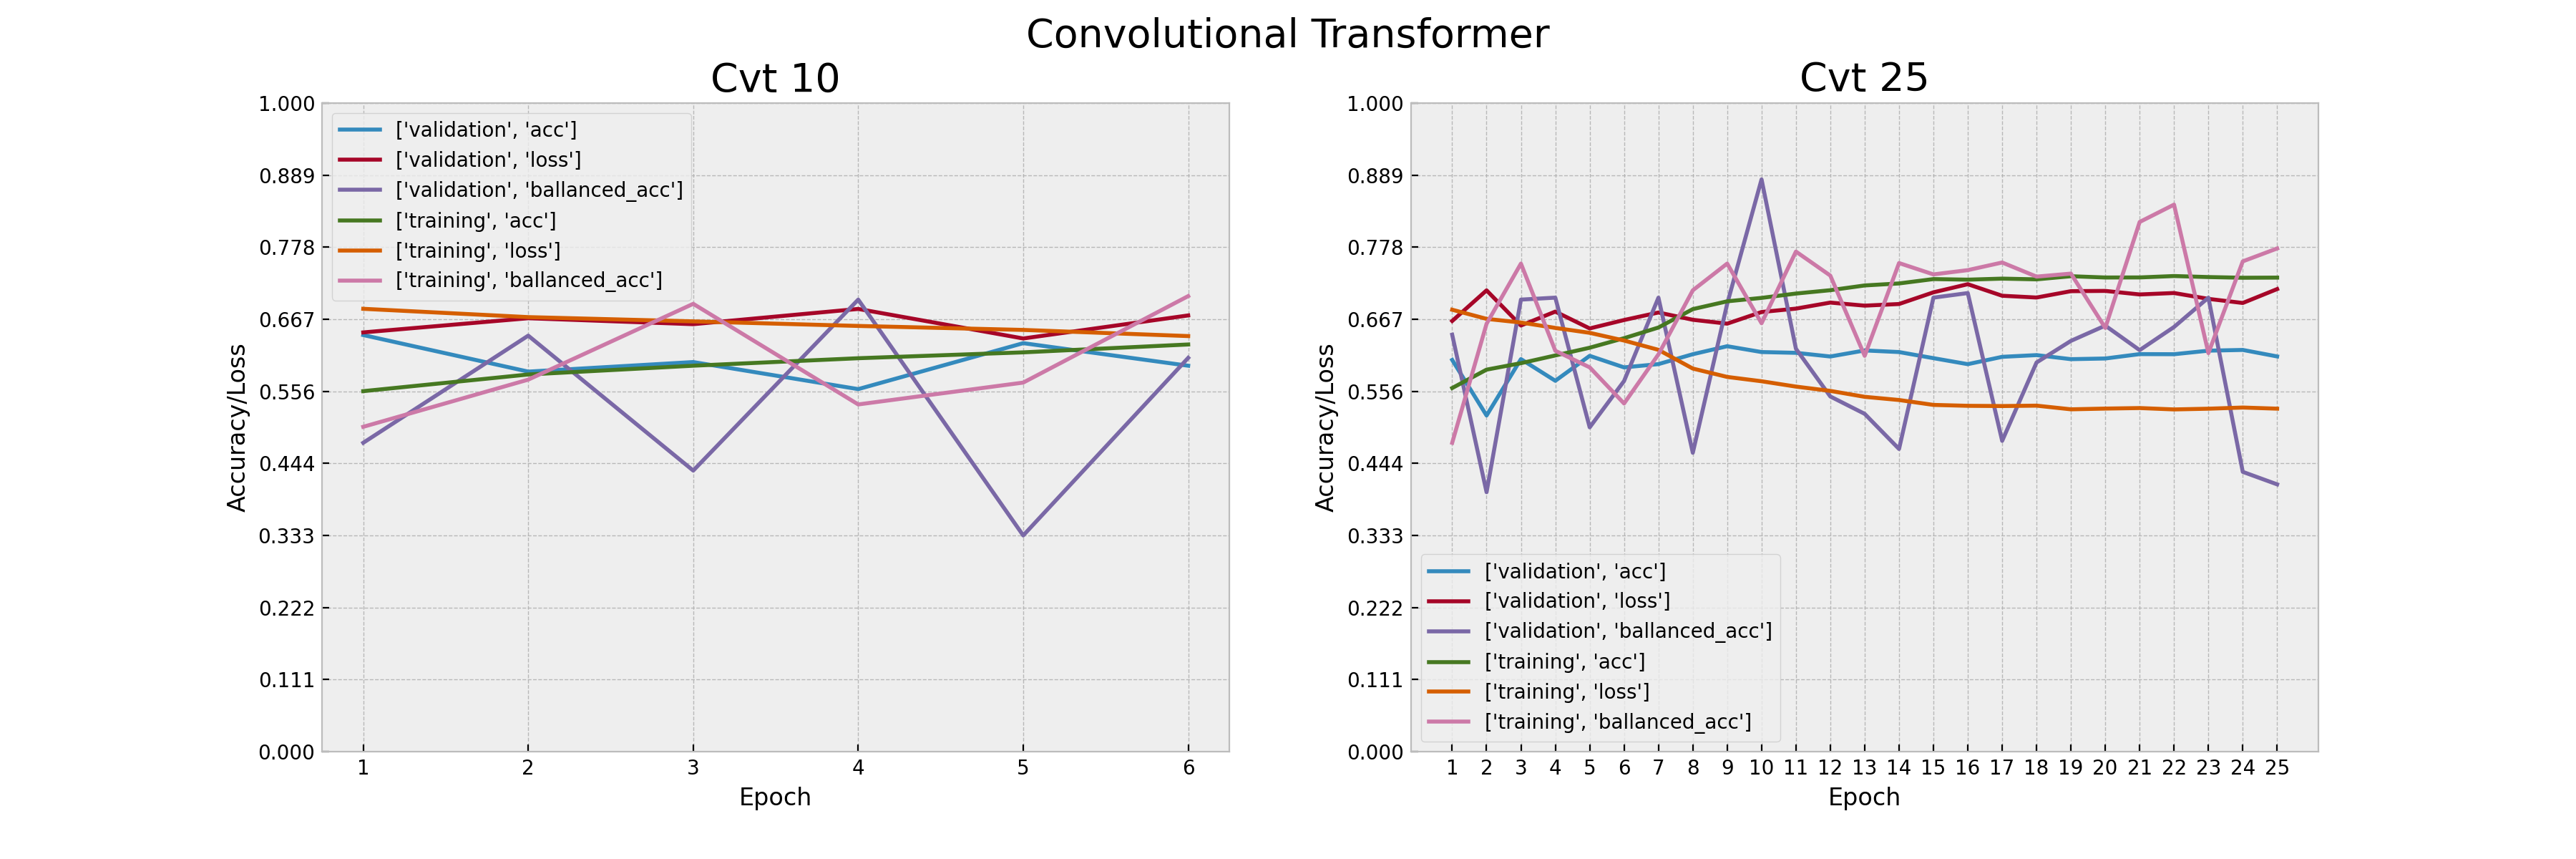
\includegraphics[width=0.9\textwidth]{figures/results_and_discussion/CVT.png}
    \caption{Hybrid Convolutional Transformer Training}
    \label{fig:CvT}
\end{figure} 

Further, it can be seen that training inference is unstable (both training and validation (balanced accuracy) vary significantly), which is consistent with observations elsewhere - often requiring a warm-up (tapering of learning rate) during initialisation. Further, given the inclusion of a data sampler, balanced accuracy does not provide a clear prediction of model accuracy and therefore subsequently trained models do not report this. \ref{fig:CvT} left.

Comparing results between CvTs and ConViTs, both without pre-training on ImageNet1k, shows erratic training performance on validation sets. 

\begin{figure}[htp!]
    \centering
    \includegraphics[width=\textwidth]{figures/results_and_discussion/ConViT Ti,S,B Without Pre-Training.png}
    \caption{ConViT Without Pre-Trainign on ImageNet1k}
    \label{fig:ConViT_non_pre_trained}
\end{figure} 

A marked improvement can be seen in the use of pre-trained models with a 5 epoch warm up, shown in \ref{fig:ConViT_non_pre_trained}, where it is also clear the model size has a bearing on validation accuracy (although this appears to be slight). 
\begin{figure}[htp!]
    \centering
    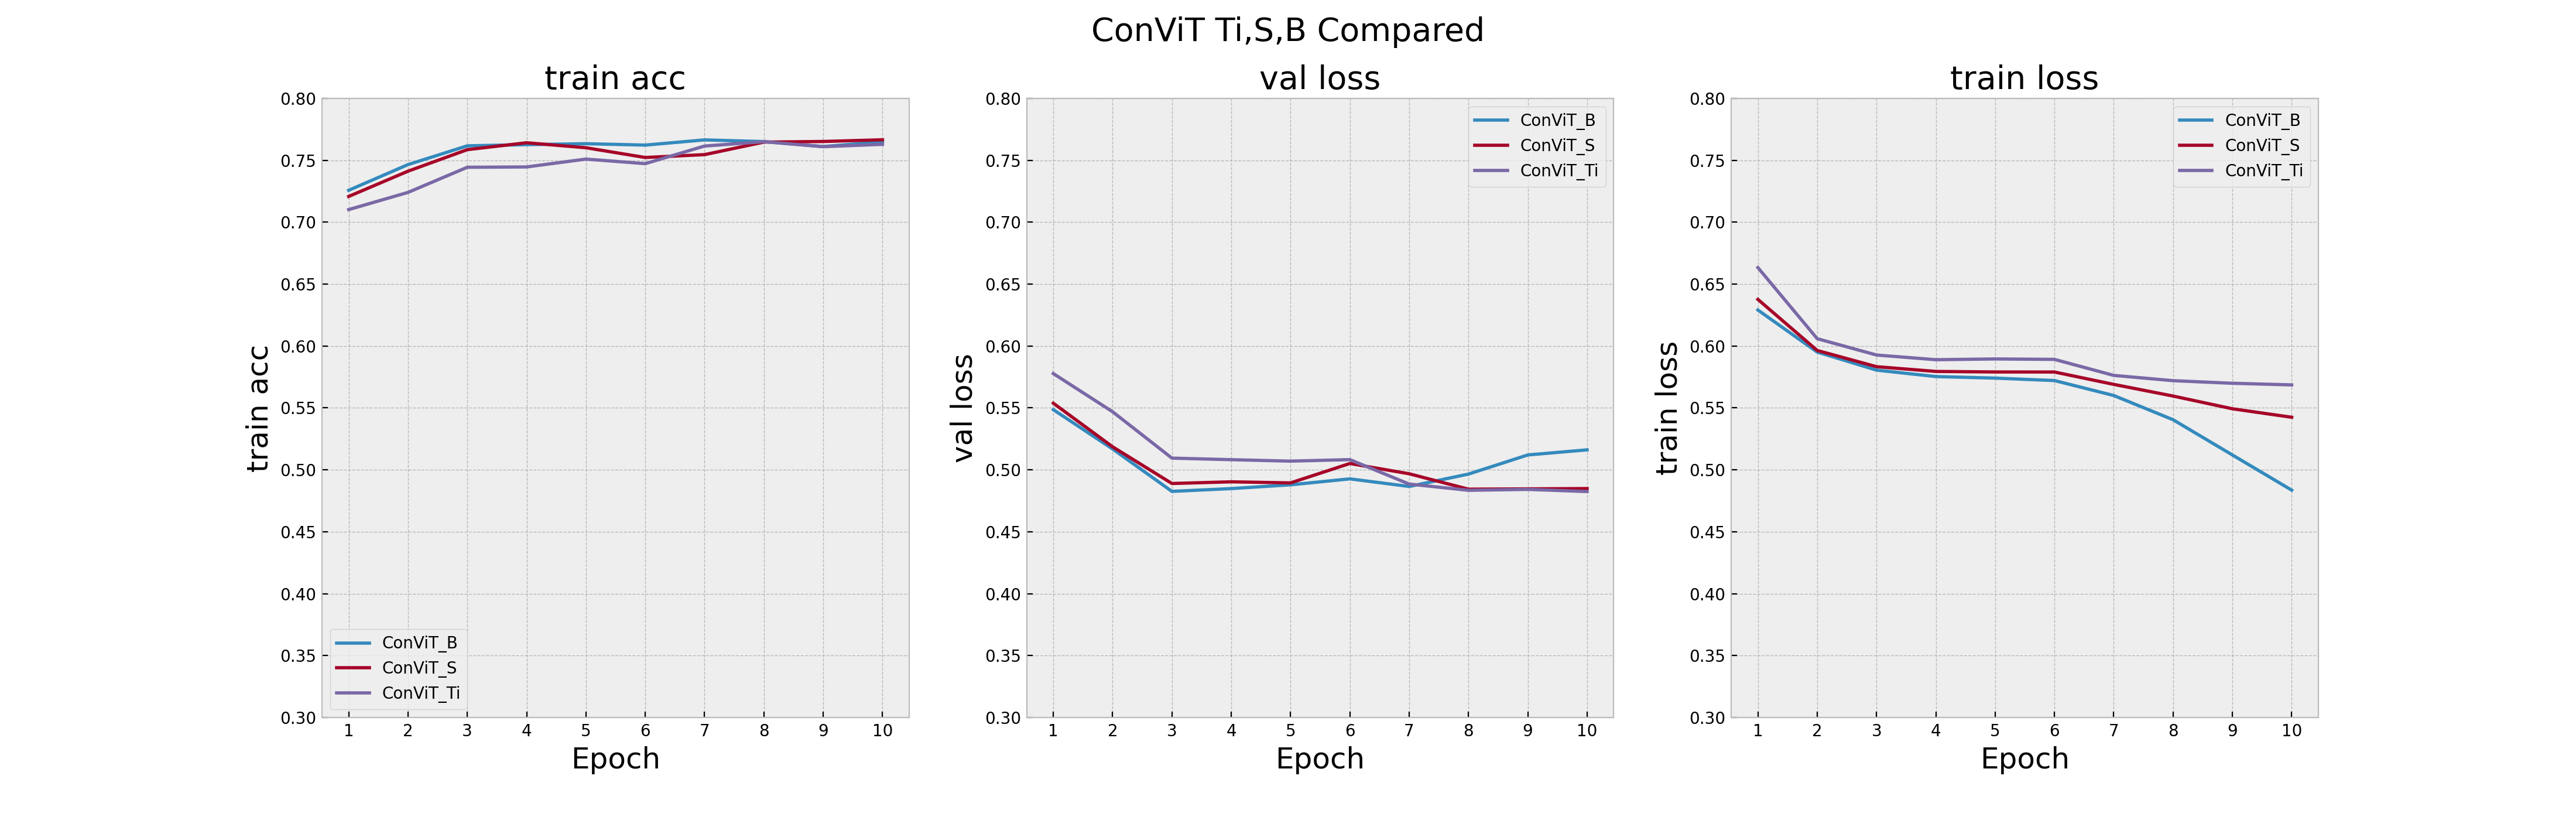
\includegraphics[width=\textwidth]{figures/results_and_discussion/ConViT Ti,S,B Compared.png}
    \caption{ConViTs With Pre-training }
    \label{fig:ConViT_pre_trained}
\end{figure} 

\subsubsection{ Hyper-Parameter Tuning and Data Augmentation}

Conducting a grid-search over learning rate and locality strength, it is clear that learn locality strength has a slight effect on model performance. Training was conducted with no warm start epochs. This shows that decreasing learning rate improves overall performance. This is shown in figure \ref{fig:ConViT_grid} left. The newly introduced hyper-parameter has some effect on overall performance.

\begin{figure}[htp!]
    \centering
    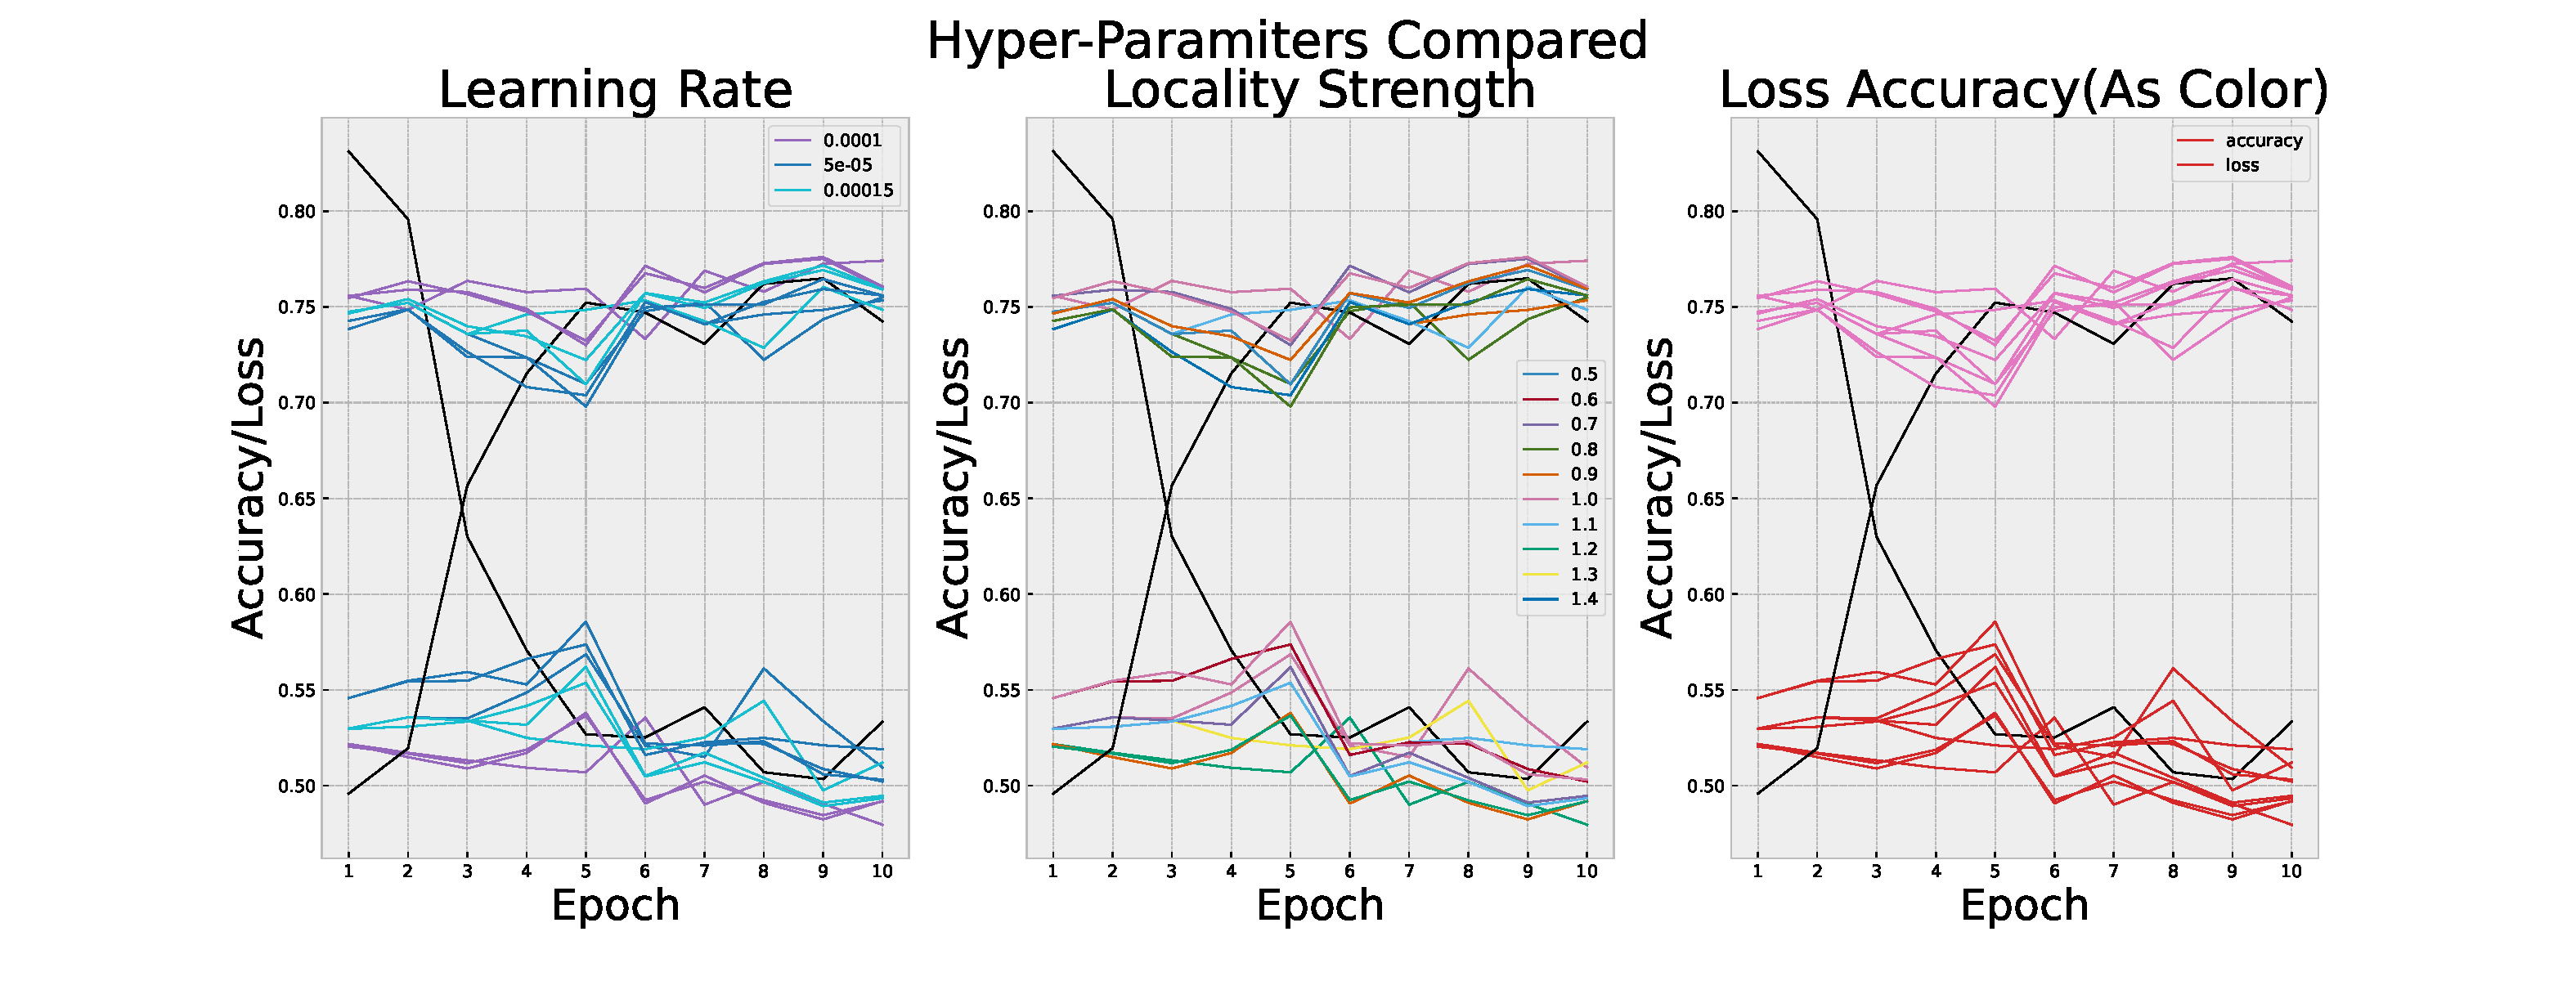
\includegraphics[width=\textwidth]{figures/results_and_discussion/hyper-params_compared.pdf}
    \caption{ConViT Ti Grid Search Between Learning Rate and Locality Strength (With Control)}
    \label{fig:ConViT_grid}
\end{figure} 

Control training, including warm up epochs, was introduced to demonstrate difference between training with and without warm starting. This is shown in black on figure \ref{fig:ConViT_grid}. This also shows that using pre-training that not using a warm start results in relatively high accuracy, with almost no training on the AVA  dataset. 

In order to compare spatial data augmentation, we performed training of salient crops where $5 \times (224 \times 224)$ sub patches of each image were taken using the attention algorithm provided by\cite{Ma2017}. This was in order to gauge how a self attention model might train on data, and whether higher resolution patches might enhance training. Training on all five sub patches separately, alongside training on all patches pooled, is shown in figure \ref{fig:sub_patching}. 

\begin{figure}
    \centering
    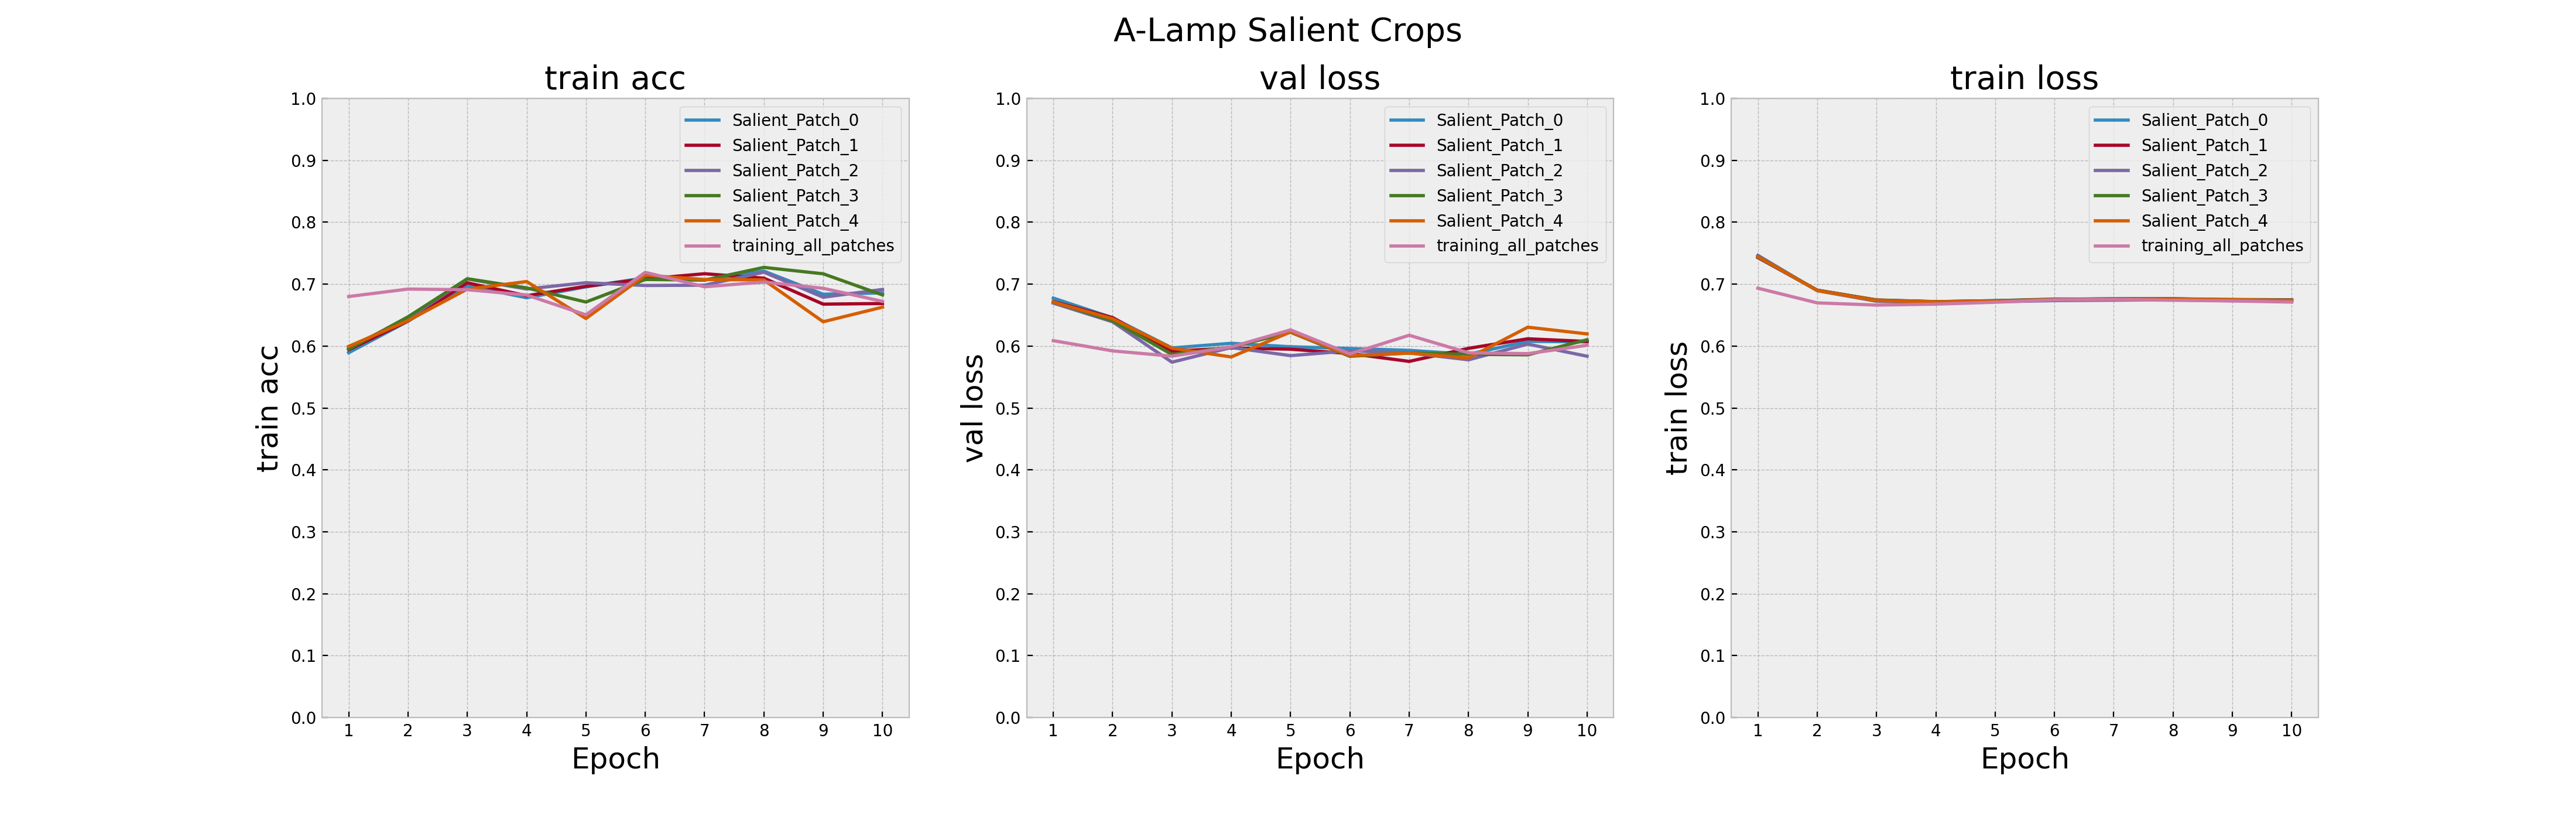
\includegraphics[width=\textwidth]{figures/results_and_discussion/A-Lamp Salient Crops.png}
    \caption{Comparison of ConViT Ti Trained on Salient Patches from A-Lamp Model \cite{Ma2017}}
    \label{fig:sub_patching}
\end{figure}
\begin{figure}
    \centering
    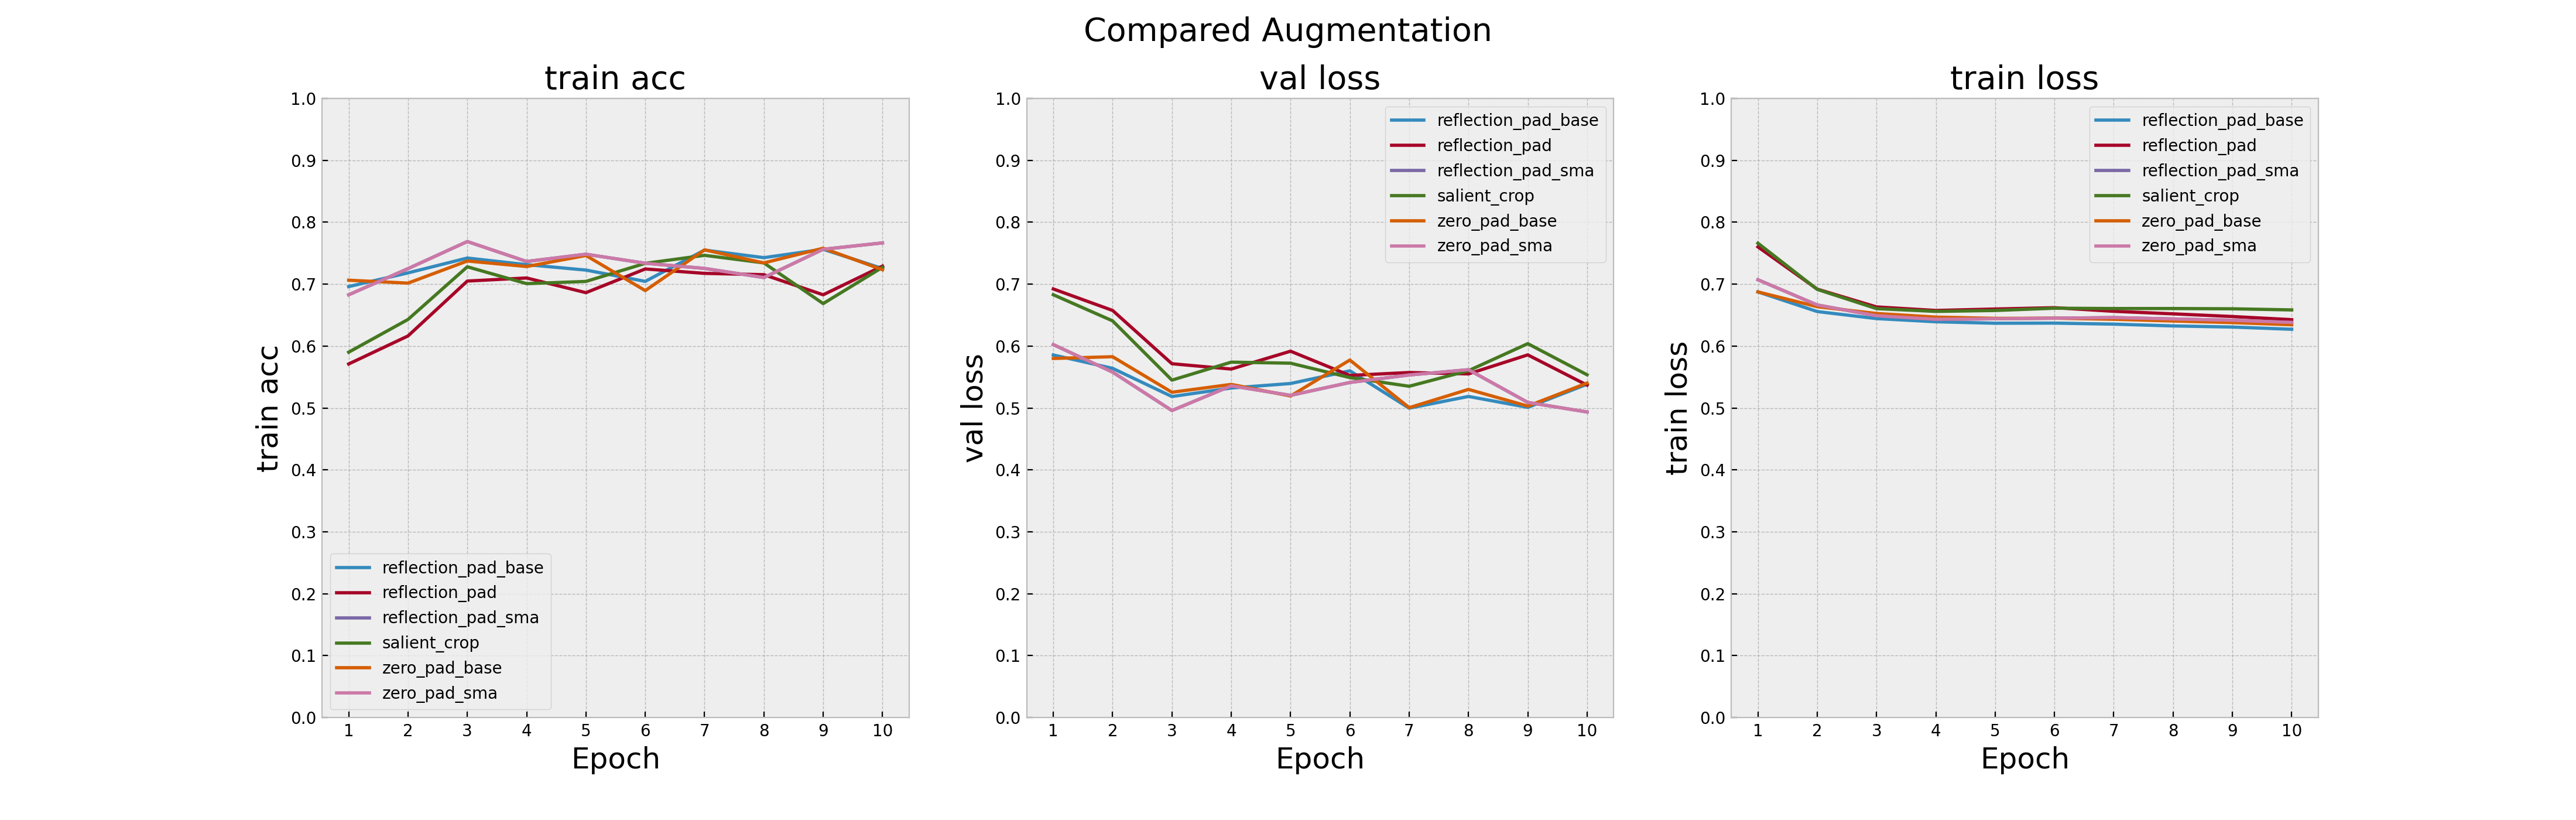
\includegraphics[width=\textwidth]{figures/results_and_discussion/Compared Augmentation.png}
    \caption{Comparison of Augmentation on ConViT B and S}
    \label{fig:my_label}
\end{figure}

Combining all demonstrates best performance, however all perform less well than a global/non cropped image, which indicates that the ConViTs are learning composition information.

We also compared training on zero-padding to square and reflection padding. The logic of this is that reflection padding maintains composition data, while reflecting the shortest edge effectively also encodes an image border.

This shows some improvement during training by reflection padding. 

\begin{table}[]
\small 
    \centering
\begin{tabular}{lcc?ccc?c}
 \toprule                                                            
{} & \multicolumn{2}{c}{Starting State} & \multicolumn{3}{c}{Augmentation} & Search         \\ 
 \toprule                                                          
{} & Pre-train  & No Pre-train                  & Reflection Pad & Zero Pad & Salient Crop  &  Grid\\
ConViT B        &                0.766          &   0.708        &       0.756   &  0.758  &   -  &  -      \\
ConViT S        &                0.767          &   0.711        &       0.769   &   0.769 &  -   &   -      \\
ConViT Ti       &                0.765          &   0.705        &       0.749   &   0.714 & 0.747& 0.776    \\
\bottomrule
\end{tabular}
    \caption{ArgMax Validation Results after 10 Epochs}
    \label{tab:results_all}
\end{table}




\subsection{Test Metrics}

Table \ref{tab:reflection} shows all results evaluated on AVA test data: 19k images on reflection padded and normalised images. Note that accuracy does not improve monotonically with model size for ConViTs, but does for ResNet models - however, F1 score does appear to obey a monotonic relationship with size of ConViT Model.

We also compared this with zero-padded images to square, as this might reflect how images are processed in the wild:

Here, each ConViT out performs in accuracy, however it is interesting to note ResNet152 out performance on balanced accuracy and F1 Score ConViT B. 
\begin{table}[ht!]
\small
    \centering
\begin{tabular}{lccccl}
\toprule
{}             &  Accuracy$\downarrow$ &  Balanced Acc.& F1     & N epochs & Weight Save Arg \\
\midrule
ViT B         &     39.96 &           26.66 &  39.93 & 10       & Last Epoch          \\
CvT           &     63.90 &           76.68 &  52.47 & 25       & Max Acc. Epoch      \\
ResNet 18 R   &     70.23 &           58.08 &  65.66 & 10       & Last Epoch          \\
ResNet 50     &     70.85 &           99.54 &  41.70 & 10       & Last Epoch          \\
ResNet 18     &     71.31 &           86.84 &  54.74 & 10       & Last Epoch          \\
ResNet 152    &     72.69 &           87.66 &  55.84 & 10       & Last Epoch          \\
ConViT Ti     &     73.17 &           95.52 &  49.58 & 10       & Last Epoch          \\
ResNet 50 R   &     74.13 &           72.06 &  65.69 & 10       & Last Epoch          \\
ConViT Ti     &     74.33 &           90.90 &  55.42 & 10       & Max Val. Acc. Epoch \\
ConViT B      &     74.58 &           85.53 &  59.65 & 10       & Last Epoch          \\
ConViT S      &     75.02 &           87.58 &  58.85 & 10       & Last Epoch          \\
ConViT S      &     75.06 &           90.22 &  56.94 & 10       & Max Val. Acc. Epoch \\
ResNet 152 R  &     75.63 &           60.32 &  70.82 & 10       & Max Val. Acc. Epoch \\
ConViT Ti R   &     76.29 &           72.33 &  68.07 & 10       & Max Val. Acc. Epoch \\
ConViT S R    &     76.29 &           72.33 &  68.07 & 10       & Max Val. Acc. Epoch \\
ConViT B      &     76.47       &         81.00 &  64.59 & 10       & Max Val. Acc. Epoch \\
ConViT B R    &     76.82       &         70.38 &  69.35 & 10       & Max Val. Acc. Epoch \\
NIMA          &     77.25       &         69.51 &  70.56 & 0        & Pre-Trained         \\
ConViT B R    & \textbf{78.11}  &\textbf{73.17} &  69.92 & 25       & Max Val. Acc. Epoch \\
MLSP          &     81.65       &         66.68 &  76.08 & 0        & Pre-Trained         \\
\bottomrule
\end{tabular}
\caption{Evaluation on Refection Padded Normalised Images Square Padded on 19k AVA Test Set}
    \label{tab:reflection}
\end{table}

We show that, when trained on best hyper parameters (from the grid search conducted [learning rate <0.0015 and locality strength 1.5]), ConViT B outperforms NIMA\cite{Talebi2018}, whose results we reproduce on their test set with a pre-trained model made available alongside their publication. Both the F1 score and balanced accuracy of MLSP\cite{Hosu2019} are lower than ours. This is in spite of the potential that training an end to end binary classifier is more challenging, with a smaller, fully connected final layer output of 2 rather than 10 (one for each MOS probability produced by normalised MOS score over 10 bins). 


One further important feature to consider is that \cite{Talebi2018, Hosu2019} both sample from much larger initial images, and we only train on $224 \times 224$ resized images. We also show a confusion matrix (each column represents the entirety of the 19k AVA Test set sample space). Here, we see that ConViT B outperforms in maintaining a high number of $TP$s while not sacrificing the the negative minority class $TN$.

\begin{table}[ht]
\tiny
    \centering
   \begin{tabular}{lrrrrrrrrr}
\toprule
{} &  ResNet 50 R &  ResNet 152 R &  ResNet 18 10 &  ConViT Ti R &  ConViT B R &  ConViT S M &  ViT B &  MLSP &  NIMA \\
\midrule
tp &         0.62 &          0.58 &          0.66 &         0.64 &        0.63 &        0.70 &   0.52 &  0.65 &  0.62 \\
tn &         0.12 &          0.18 &          0.05 &         0.13 &        0.14 &        0.05 &   0.08 &  0.17 &  0.15 \\
fp &         0.09 &          0.13 &          0.05 &         0.08 &        0.08 &        0.01 &   0.19 &  0.06 &  0.08 \\
fn &         0.16 &          0.11 &          0.23 &         0.16 &        0.15 &        0.24 &   0.20 &  0.12 &  0.15 \\
\bottomrule
\end{tabular}

    \caption{Confusion Metrics on 19k AVA Test-Set 19k }
    \label{tab:Cofusion Metrics}
\end{table}


Table \ref{tab:Model Types} shows nomenclature used in tables (\ref{tab:reflection}, \ref{tab:Cofusion Metrics}), as models performed differently according to whether zero-padding or reflection padding were used during data augmentation. We also show type number of layers and dimension of resized images. 

\begin{table}[ht!]
\small 
    \centering
   \begin{tabular}{llllc}
\toprule
{}         & Augment             & Layers                    & Type            & Dimensions      \\
\midrule
ResNet 18  Z & Zero Pad      & 18 Residual    &  CNN                           & $224 \times 244$\\
ResNet 50  Z & Zero Pad      & 50 Residual    &  CNN                           & $224 \times 244$\\
ResNet 152 Z & Zero Pad      & 152 Residual   &  CNN                           & $224 \times 244$\\
ConViT Ti  Z & Zero Pad      & $12 \times 3$  & Conv. Vision Transformer       & $224 \times 244$\\
ConViT S   Z & Zero Pad      & $12 \times 6$  & Conv. Vision Transformer       & $224 \times 244$\\
ConViT B   Z & Zero Pad      & $12\times 12$  & Conv. Vision Transformer       & $224 \times 244$\\
ResNet 18  R & Reflect Pad   & 18 Residual    &  CNN                           & $224 \times 244$\\
ResNet 50  R & Reflect Pad   & 50 Residual    &  CNN                           & $224 \times 244$\\
ResNet 152 R & Reflect Pad   & 152 Residual   &  CNN                           & $224 \times 244$\\
ConViT Ti  R & Reflect Pad   & $12 \times 3$  & Conv. Vision Transformer       & $224 \times 244$\\
ConViT S   R & Reflect Pad   & $12 \times 6$  & Conv. Vision Transformer       & $224 \times 244$\\
ConViT B   R & Reflect Pad   & $12\times 12$  & Conv. Vision Transformer       & $224 \times 244$\\
ViT B      R & Reflect Pad   & $12\times 12$  & Vision Transformer             & $224 \times 244$\\
CvT        R & Reflect Pad   & $3\times 10$   & Conv. Vision Transformer       & $224 \times 244$\\
 
\bottomrule
\end{tabular}
    \caption{Number Parameters and Training Time Per Epoch 230k Images on 1 GPU- batch size 10 Inference on 19k Images on AVA dataset}
    \label{tab:Model Types}
\end{table}

\section{Exclusive Set Analysis}
\label{sec:exclusive set}

This section shows images from the subsets shown in Table \ref{tab:unique}. These images are a complement set of the union of all other model inferences on the 19k image AVA test set, $M= \overline{\cup}_{i=1}^{n}F_{i}$ where $F$ is all other models.  This is performed for each model and each inference type $\in \{tp,tn,fp,fn\}$. The results are shown in table \ref{tab:unique}, we compute this for the best performing model of each type. This shows as a discreet value, the number of images where a single model over or under performs against all the others in the entirety of the 19k.  

\begin{table}[ht!]
\small 
    \centering
\begin{tabular}{lrrrr}
\toprule
{} &    tn &    fp &    fn &     tp \\
\midrule
ResNet 50 R  &   131 &    17 &   408 &      7 \\
ResNet 152 R &   343 &     2 &   599 &      1 \\
ResNet 18 10 &    52 &   122 &   286 &     13 \\
ConViT Ti R  &    86 &     3 &   170 &      1 \\
ConViT B R   &   129 &     9 &   201 &      4 \\
ConViT S R   &     5 &    76 &     9 &     24 \\
ViT B        &   341 &   157 &  2422 &     18 \\
\bottomrule
\end{tabular}
    \caption{Number of Unique Images by Confusion Metric Categories}
    \label{tab:unique}
\end{table}

An interesting observation is that ViT, despite performing poorly overall, still correctly identifies a significant number of images that are challenging for other models. Overall, ResNets have far more false negatives where they alone under-performed. This is an important observation, as this is for the minority class. Here, one might consider whether this gap would grow with the availability of more data. 





\section{Qualitative Results}
\label{sec:Qualitative Results}
We show images from the test 19k test set - which are identified by each network in $\in \{tp,tn,fp,fn\}$ - and are members of the exclusive sets shown in table \ref{tab:unique}. This may provide insight into the types of images that each network is performing best and worst (that is unique to that each networks inference). Images are chosen at random from each exclusive set. This is to provide insight into how each network is selecting attributes that may be visible to the human eye.  It is clear from the MOS score that these images are generally from the ambiguous range of MOS. 

\subsection{ResNets and ConViTs True Negative}


\begin{figure}[ht!]
    
    \subfloat[True Negatives Only Identified By ConViT]{\includegraphics[width=0.333\textwidth]{figures/results_and_discussion/qualitative_results/ConViT B TN.png} \label{fig:ConViT_B_TN}}
     \subfloat[ConViT S True Negative Images]{\includegraphics[width=0.333\textwidth]{figures/results_and_discussion/qualitative_results/ConViT S TN.png}
     \label{fig:ConViT_S_TN}}
     \subfloat[ConViT Ti True Negative Images]{\includegraphics[width=0.333\textwidth]{figures/results_and_discussion/qualitative_results/ConViT Ti TN.png}
     \label{fig:ConViT_Ti_TN}}
    \vfill  
    \subfloat[ResNet 152 True Negative Images]{\includegraphics[width=0.333\textwidth]{figures/results_and_discussion/qualitative_results/resnet 152 TN.png}
    \label{fig:ResNet_152_TN}}
    \subfloat[ResNet 50 True Negative Images]{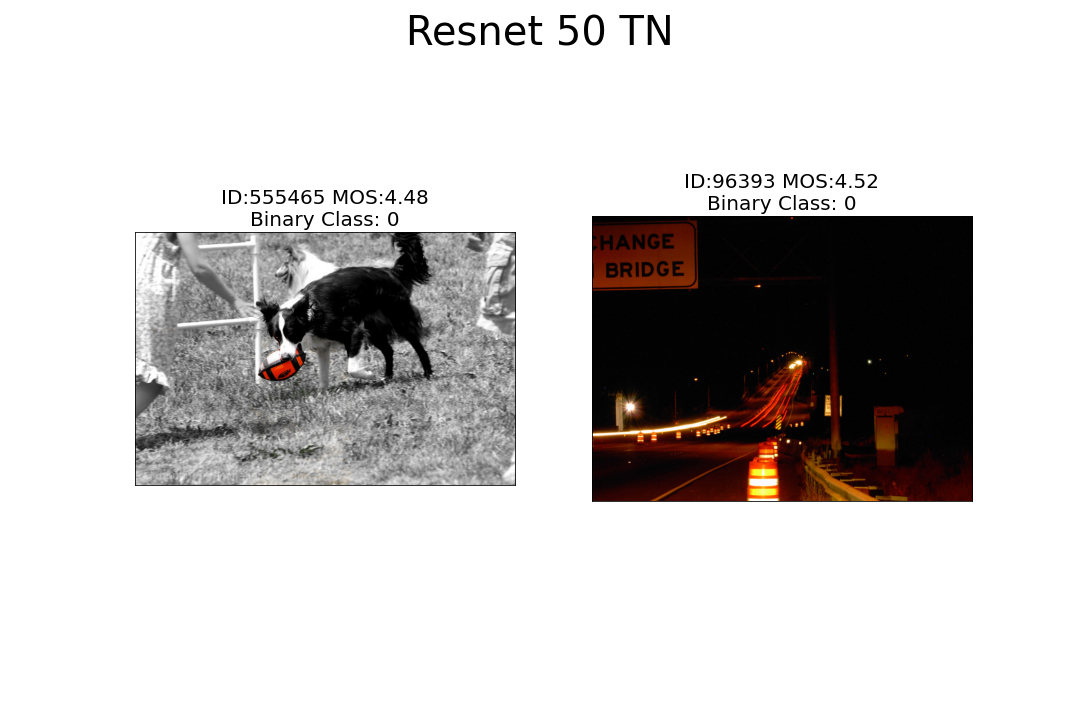
\includegraphics[width=0.333\textwidth]{figures/results_and_discussion/qualitative_results/Resnet 50 TN.png}\label{fig:ResNet_50_TN}}
    \subfloat[ResNet 18 True Negative Images]{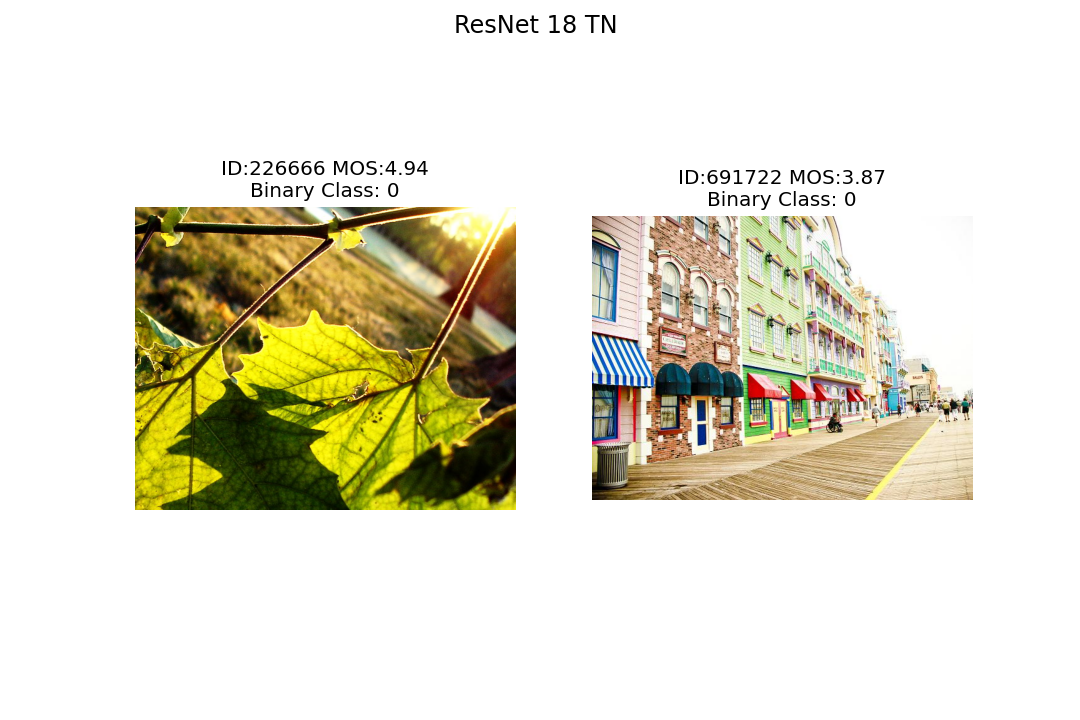
\includegraphics[width=0.333\textwidth]{figures/results_and_discussion/qualitative_results/ResNet 18 TN}, \label{fig:ResNet_18_TN}}
    \caption{Examples of Exclusive True Negatives Predictions by Each Network (Exclusive Set) on AVA Test Set}
    \label{fig:true_negative}
\end{figure}

ConViTs (\ref{fig:ConViT_B_TN}, \ref{fig:ConViT_S_TN}, \ref{fig:ConViT_Ti_TN}) appear to pay more attention to composition information, where as ResNets - shown in figures ( \ref{fig:ResNet_152_TN}, \ref{fig:ResNet_50_TN}, \ref{fig:ResNet_18_TN})- appear to predict better where attributes such as good lighting and colour harmony are distinguishing features for images in the ambiguous range.

\subsection{ResNets and ConViTs True Positive Images}
\label{qualitative positives}

ConViT models appear to be less able to resolve positive class images that are not identified elsewhere. Again, it seems clear that interplay between composition and salient objects/distinguishing features, where figures (\ref{fig:ConViT_B_TP}, \ref{fig:ConViT_S_TP},\ref{fig:ConViT_Ti_TP}) appear to show some semantic class ambiguity \ref{fig:ConViT_Ti_TP}. Left shows an animal made of grass/leaves and \ref{fig:ConViT_B_TP} shows an image of parking meters that have eyes.

\begin{figure}[ht!]
    
    \subfloat[True Positives Only Identified By ConViT]{\includegraphics[width=0.333\textwidth]{figures/results_and_discussion/qualitative_results/ConViT B TP.png} \label{fig:ConViT_B_TP}}
     \subfloat[ConViT S True Positive Images]{\includegraphics[width=0.333\textwidth]{figures/results_and_discussion/qualitative_results/ConViT S TP.png}
     \label{fig:ConViT_S_TP}}
     \subfloat[ConViT Ti True Positive Images]{\includegraphics[width=0.333\textwidth]{figures/results_and_discussion/qualitative_results/ConViT Ti TP.png}
     \label{fig:ConViT_Ti_TP}}
    \vfill  
    \subfloat[ResNet 152 True Positive Images]{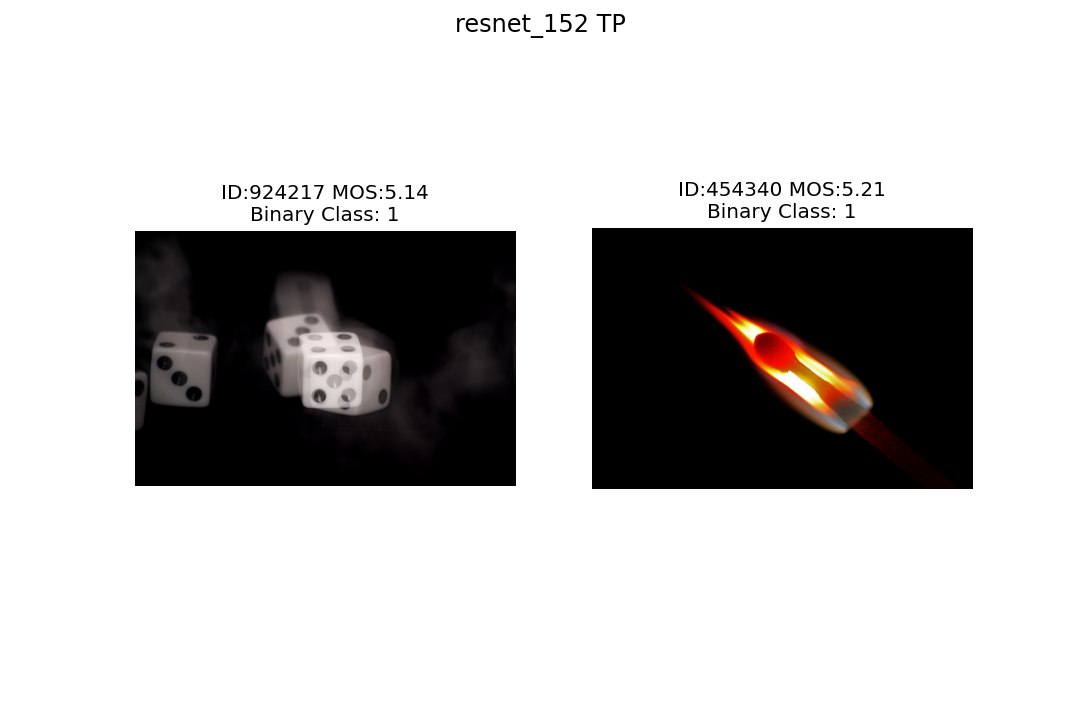
\includegraphics[width=0.333\textwidth]{figures/results_and_discussion/qualitative_results/resnet_152 TP.png}
    \label{fig:ResNet_152_TP}}
    \subfloat[ResNet 50 True Positive Images]{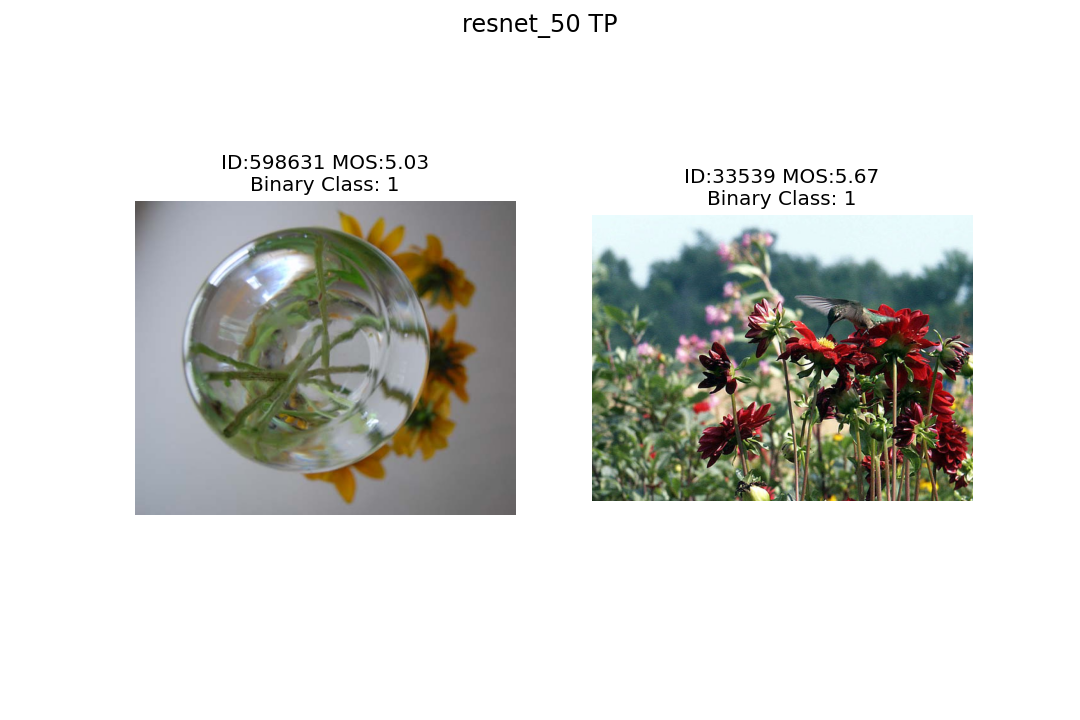
\includegraphics[width=0.333\textwidth]{figures/results_and_discussion/qualitative_results/resnet_50 TP.png}\label{fig:ResNet_50_TP}}
    \subfloat[ResNet 18 True Negative Imgaes]{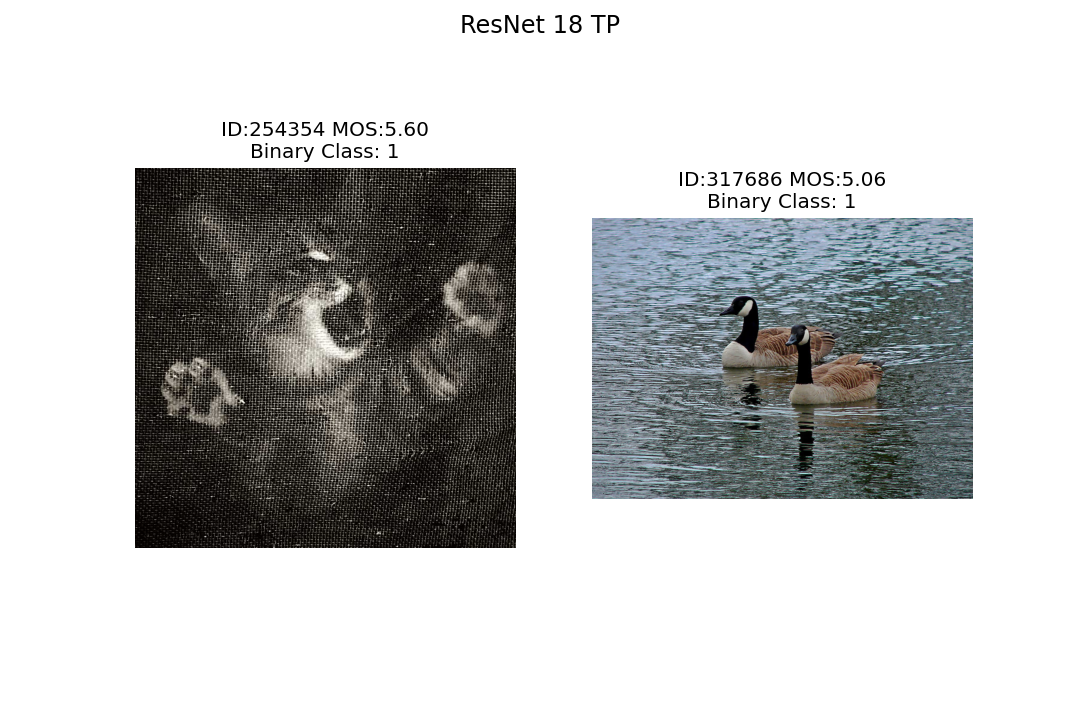
\includegraphics[width=0.333\textwidth]{figures/results_and_discussion/qualitative_results/ResNet 18 TP.png}, \label{fig:ResNet_18_TP}}
    \caption{Examples of Exclusive True Positive Predictions by Each Network (Exclusive Set) on AVA Test Set}
    \label{fig:true_positive}

\end{figure}
\subsection{ResNets and ConViTs False Negative Images}
\label{qualitative false negative}

ConViT $FN$s are shown in figures (\ref{fig:ConViT_B_FN}, \ref{fig:ConViT_S_FN},\ref{fig:ConViT_Ti_FN}) and appear to falsely rate images as negative with a bias again towards high level semantic information, in contrast with ResNets' $FN$s shown in  figures(\ref{fig:ResNet_152_FN}, \ref{fig:ResNet_50_FN}, \ref{fig:ResNet_18_FN}).

\begin{figure}[ht!]
    
    \subfloat[ConVit B Only False Negative ]{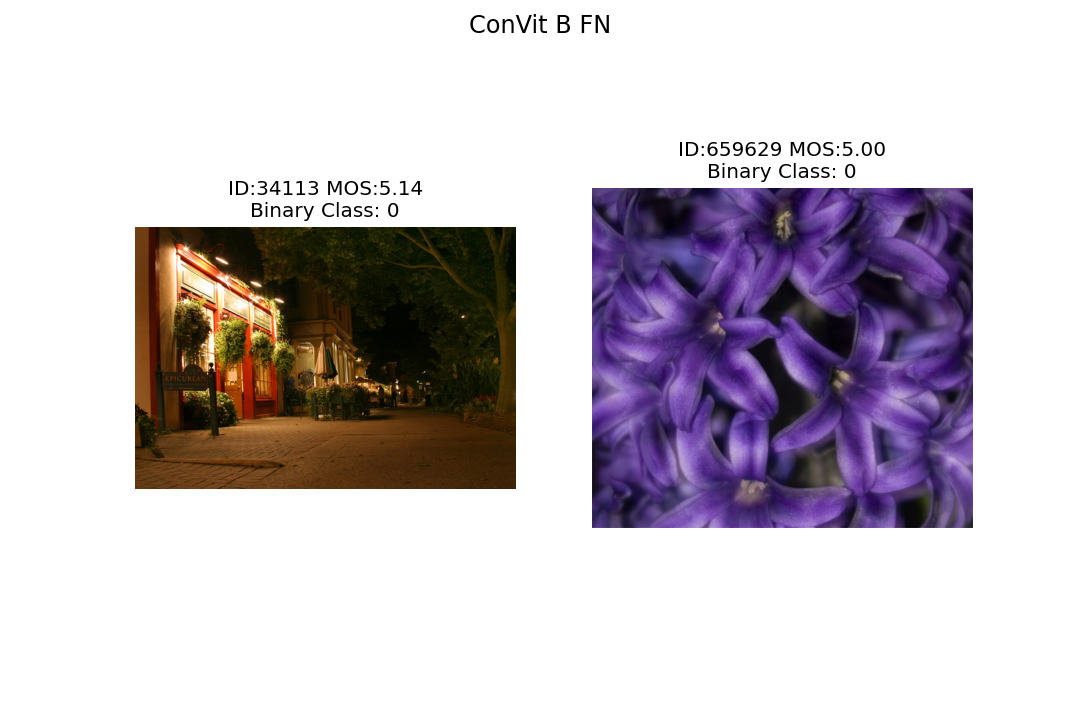
\includegraphics[width=0.333\textwidth]{figures/results_and_discussion/qualitative_results/false_negative/ConVit B FN.png} \label{fig:ConViT_B_FN}}
     \subfloat[ConViT S Only False Negative Images]{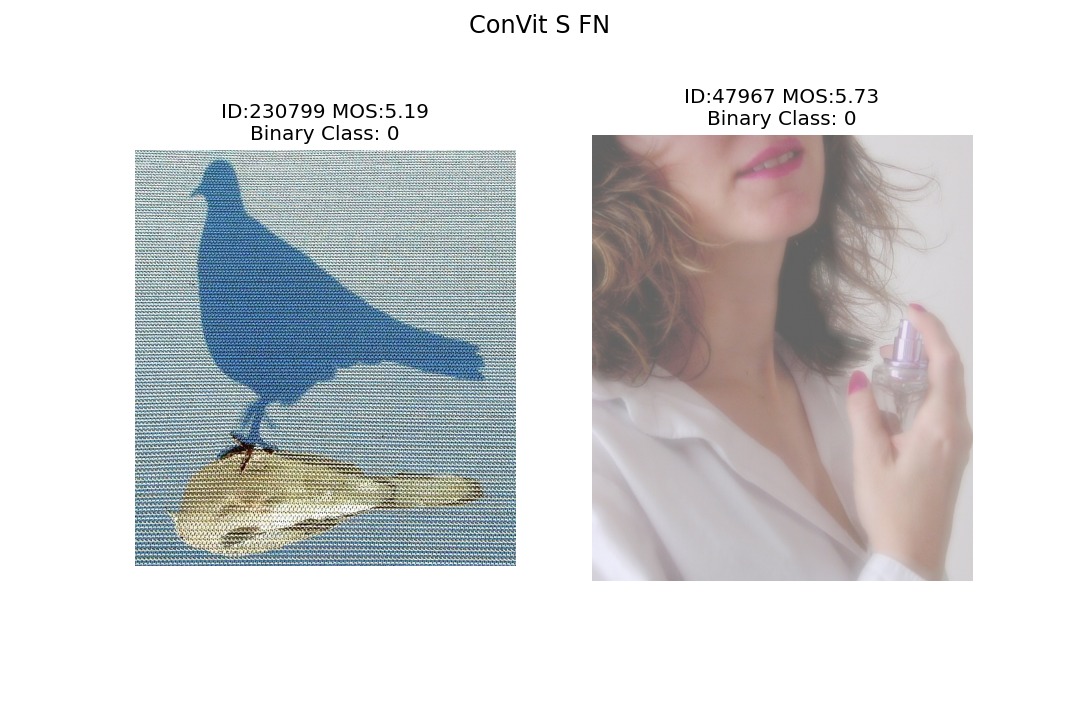
\includegraphics[width=0.333\textwidth]{figures/results_and_discussion/qualitative_results/false_negative/ConVit S FN.png}
     \label{fig:ConViT_S_FN}}
     \subfloat[ConViT Ti Only False Negative Images]{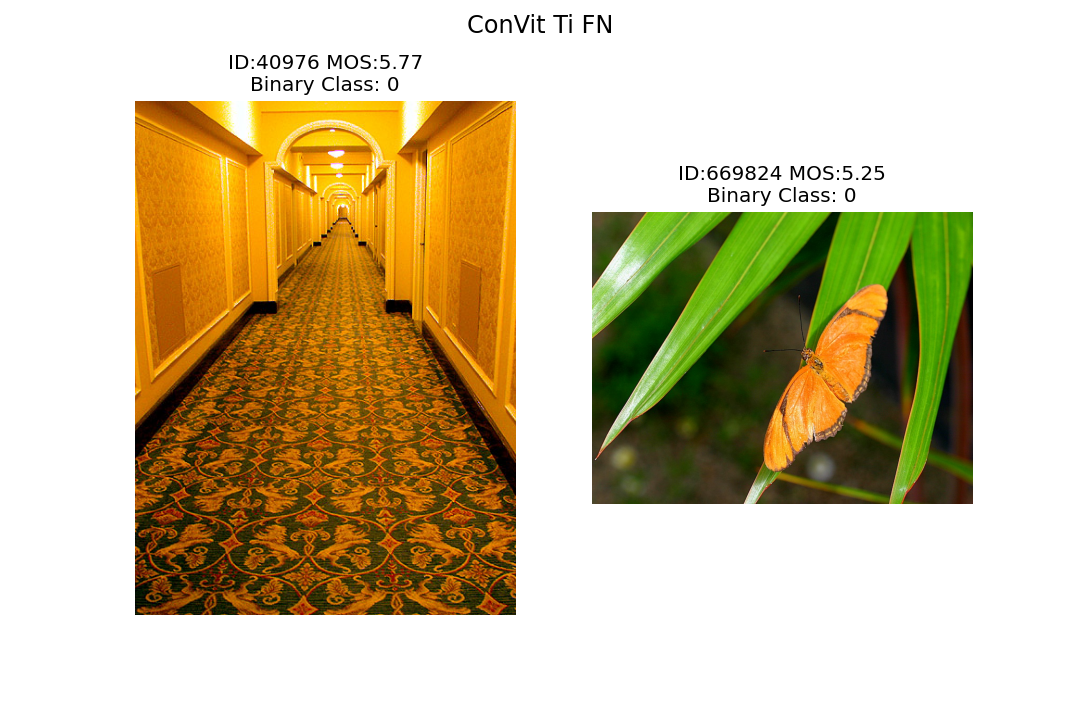
\includegraphics[width=0.333\textwidth]{figures/results_and_discussion/qualitative_results/false_negative/ConVit Ti FN.png}
     \label{fig:ConViT_Ti_FN}}
    \vfill  
    \subfloat[ResNet 152 Only False Negative Images]{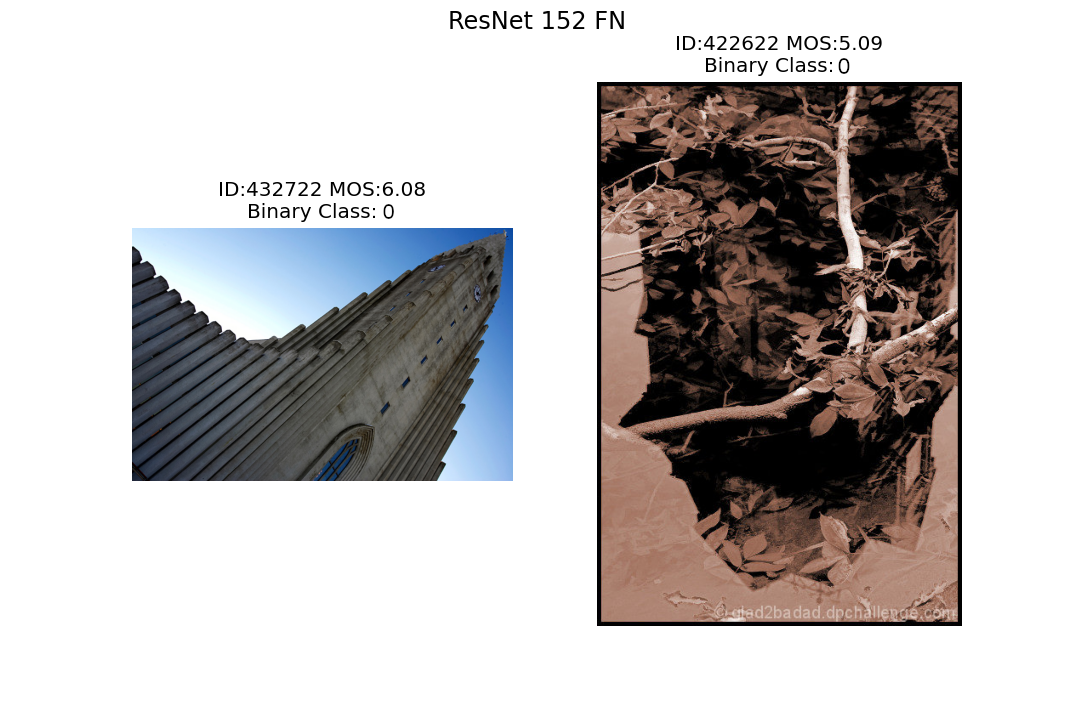
\includegraphics[width=0.333\textwidth]{figures/results_and_discussion/qualitative_results/false_negative/ResNet 152 FN.png}
    \label{fig:ResNet_152_FN}}
    \subfloat[ResNet 50 Only False Negative Images]{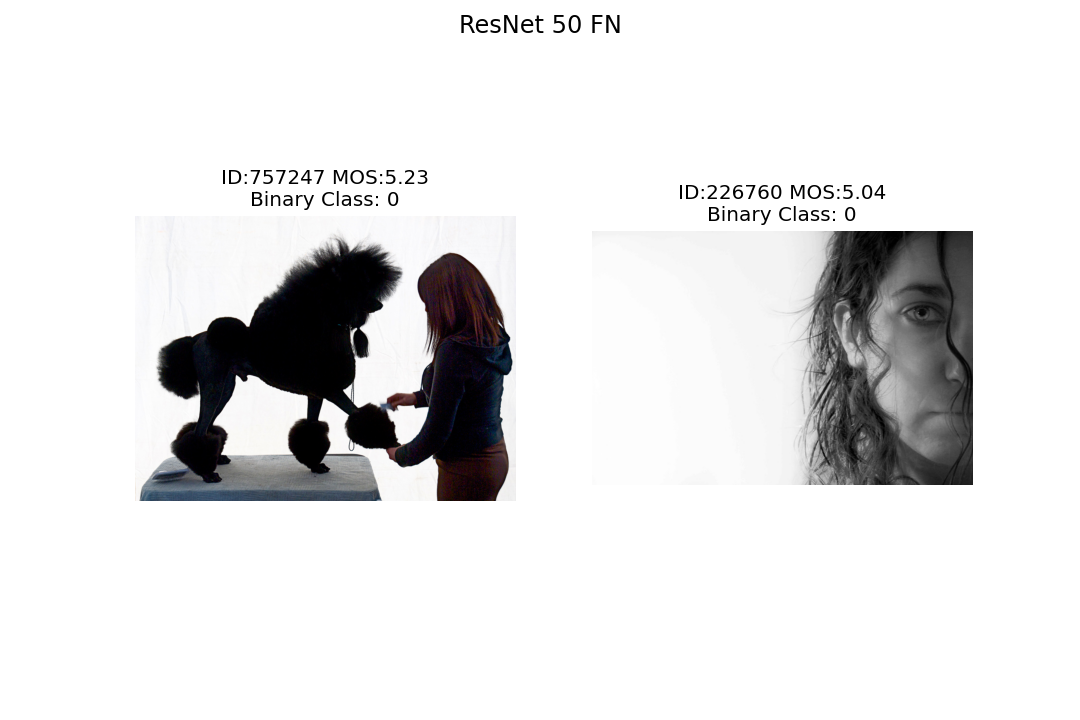
\includegraphics[width=0.333\textwidth]{figures/results_and_discussion/qualitative_results/false_negative/ResNet 50 FN.png}\label{fig:ResNet_50_FN}}
    \subfloat[ResNet 18 Only False Negative Imgaes]{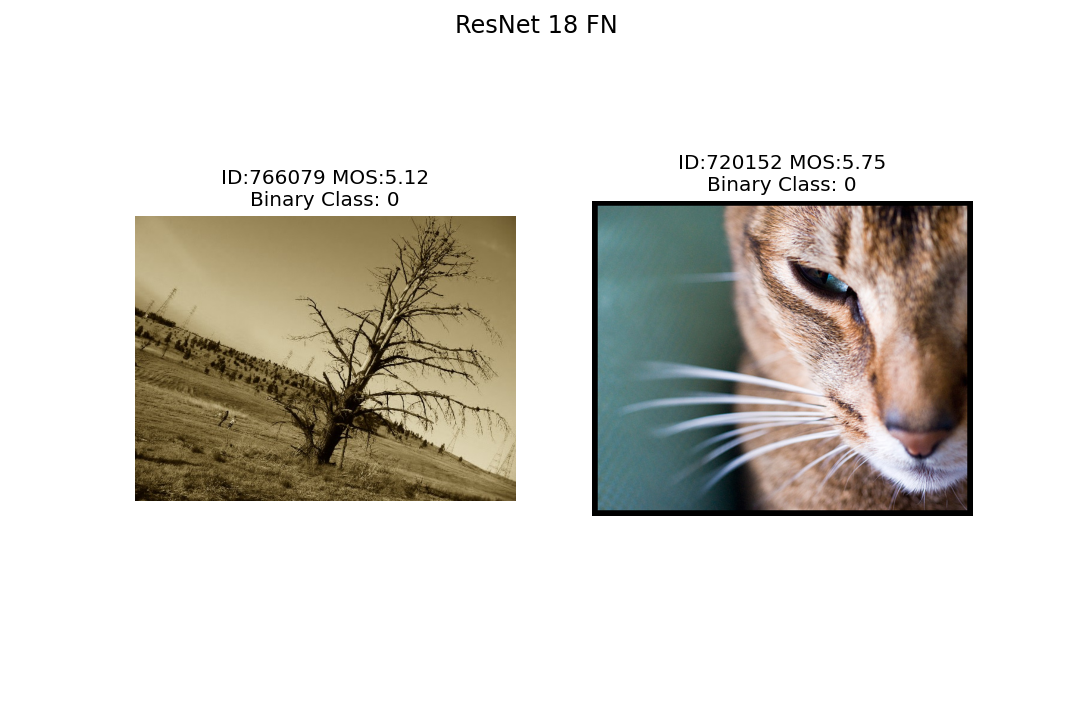
\includegraphics[width=0.333\textwidth]{figures/results_and_discussion/qualitative_results/false_negative/ResNet 18 FN .png}, \label{fig:ResNet_18_FN}}
    \caption{Examples of Exclusive False Negative Predictions by Each Network (Exclusive Set) on AVA Test Set }
    \label{fig:true_positive}

\end{figure}
\subsection{ResNets and ConViTs False Positive Images}
\label{qualitative false positive}
\begin{figure}[ht!]
    \subfloat[ConViT B Only False Positive]{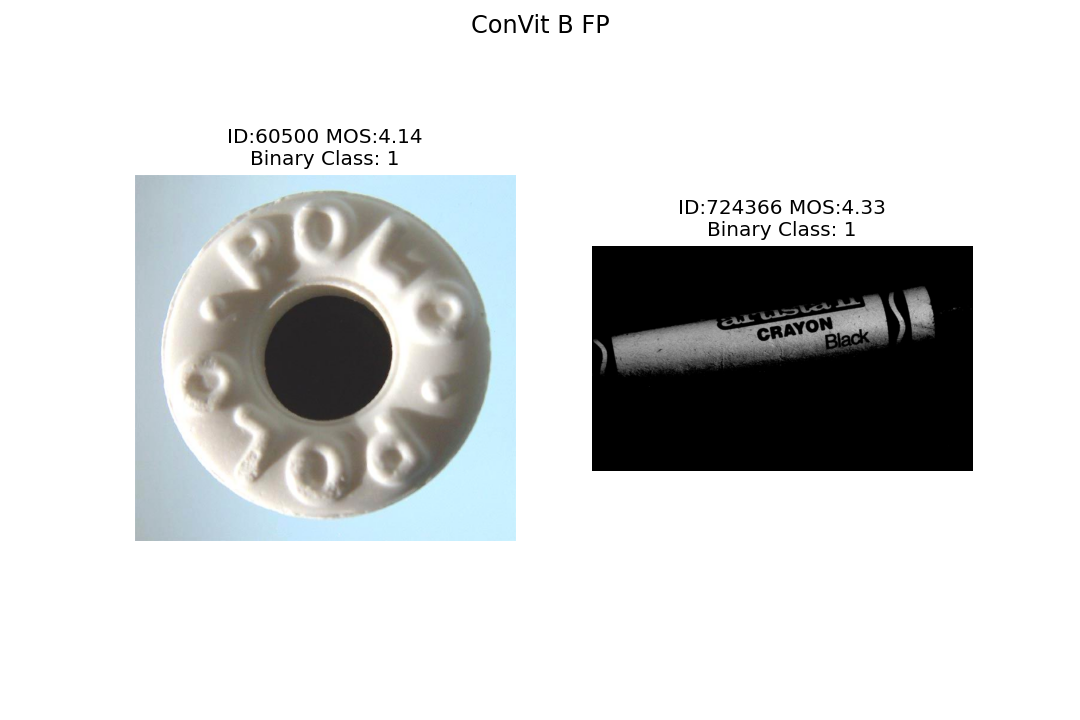
\includegraphics[width=0.333\textwidth]{figures/results_and_discussion/qualitative_results/false_positive/ConVit B FP.png} \label{fig:ConViT_B_FP}}
     \subfloat[ConViT S Only False Positive]{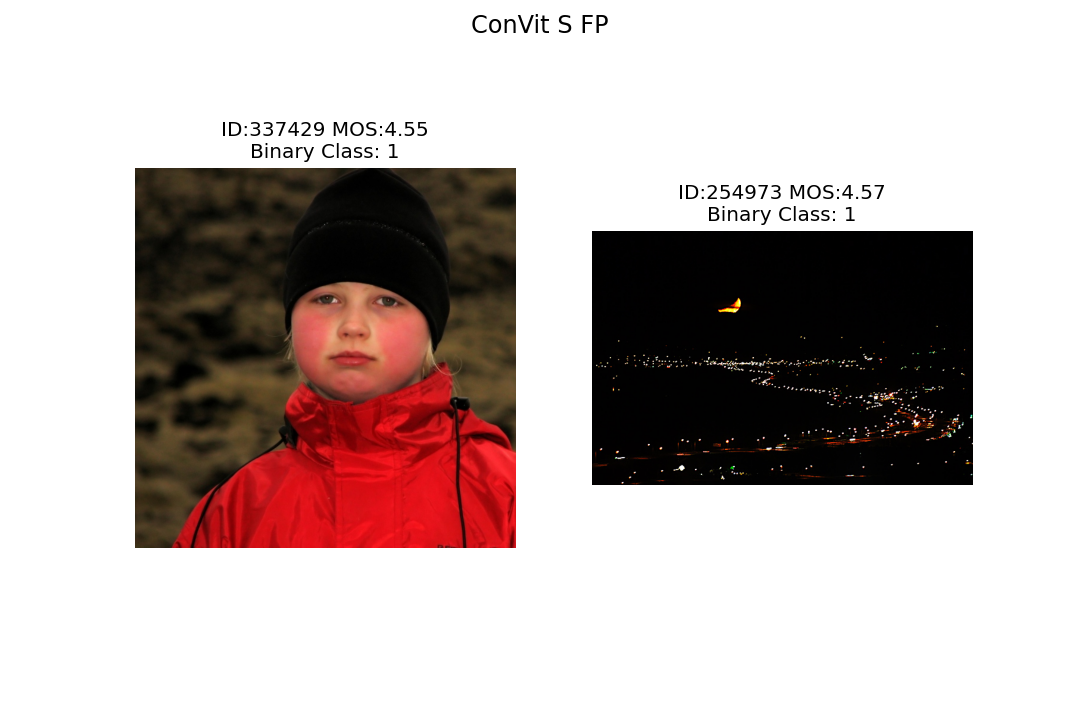
\includegraphics[width=0.333\textwidth]{figures/results_and_discussion/qualitative_results/false_positive/ConVit S FP.png}
     \label{fig:ConViT_S_FP}}
     \subfloat[ConViT Ti Only False Positive]{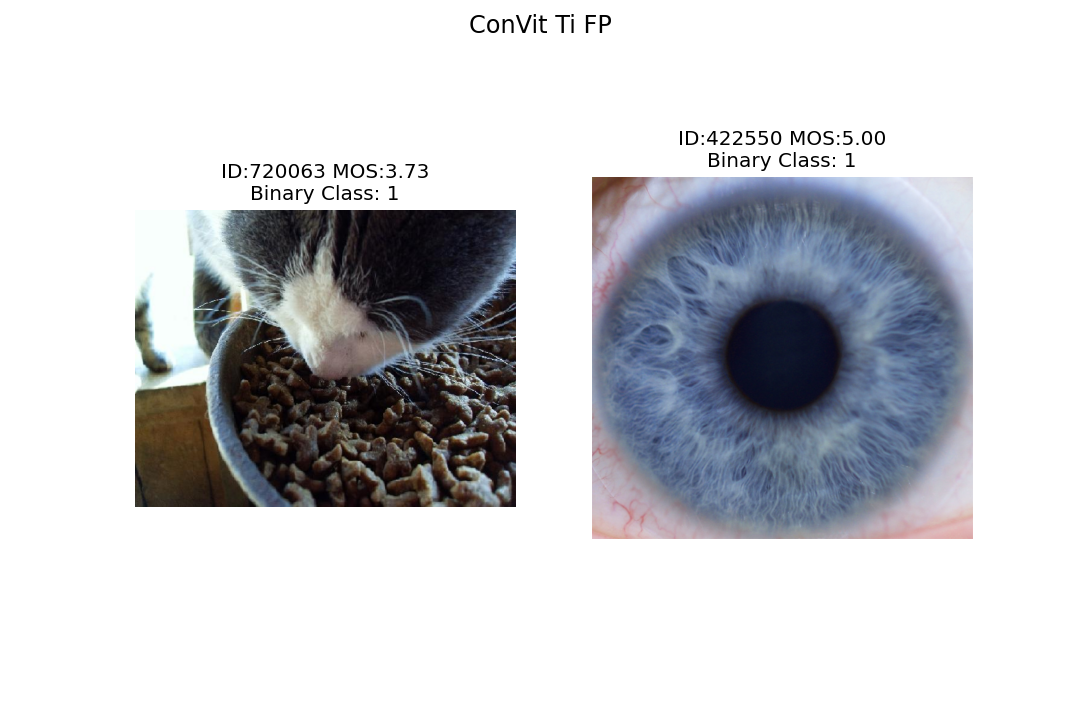
\includegraphics[width=0.333\textwidth]{figures/results_and_discussion/qualitative_results/false_positive/ConVit Ti FP.png}
     \label{fig:ConViT_Ti_FP}}
    \vfill  
    \subfloat[ResNet 152 Only False Positives]{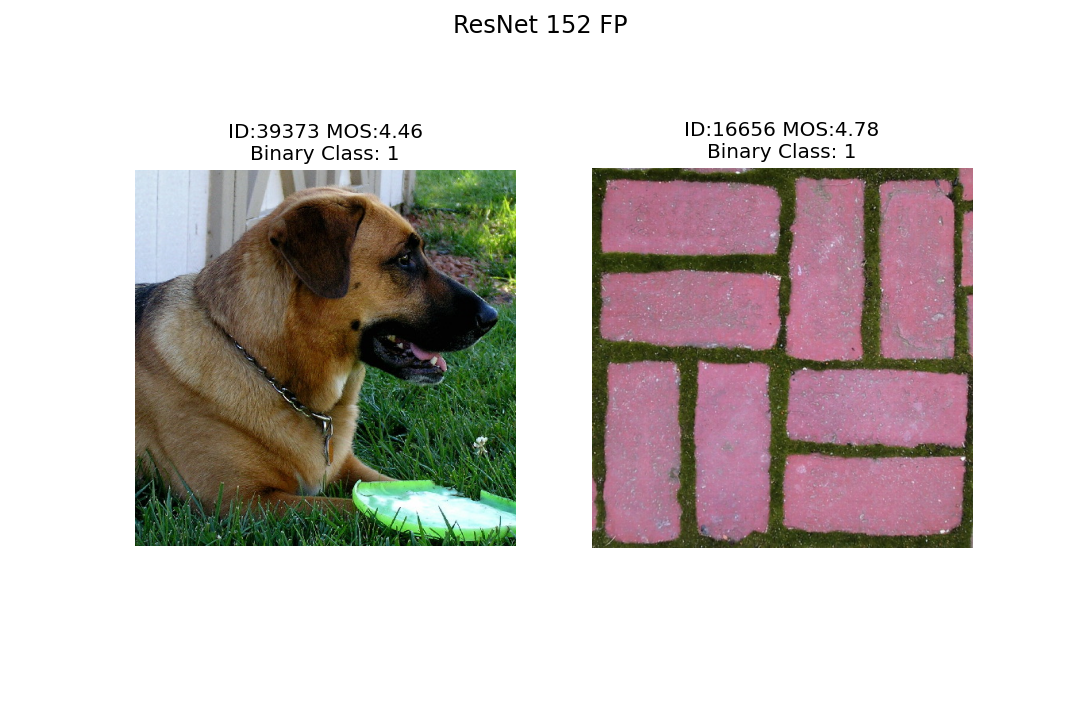
\includegraphics[width=0.333\textwidth]{figures/results_and_discussion/qualitative_results/false_positive/ResNet 152 FP.png}
    \label{fig:ResNet_152_FP}}
    \subfloat[ResNet 50 Only False Positive]{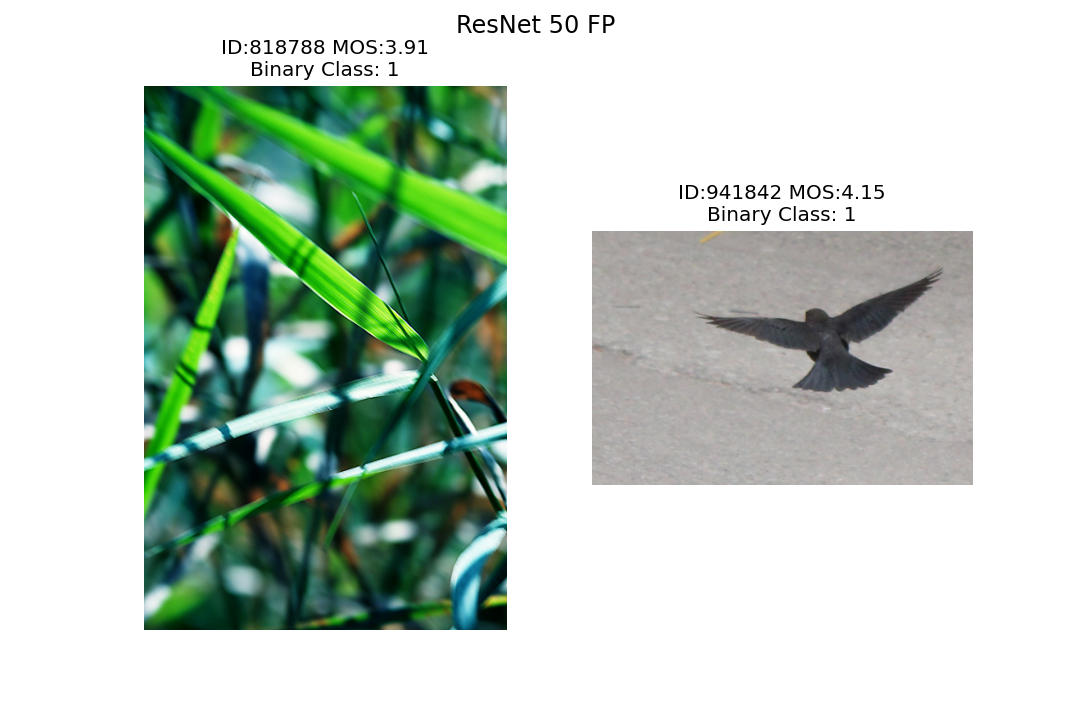
\includegraphics[width=0.333\textwidth]{figures/results_and_discussion/qualitative_results/false_positive/ResNet 50 FP.png}\label{fig:ResNet_50_FP}}
    \subfloat[ResNet 18 Only False Positive]{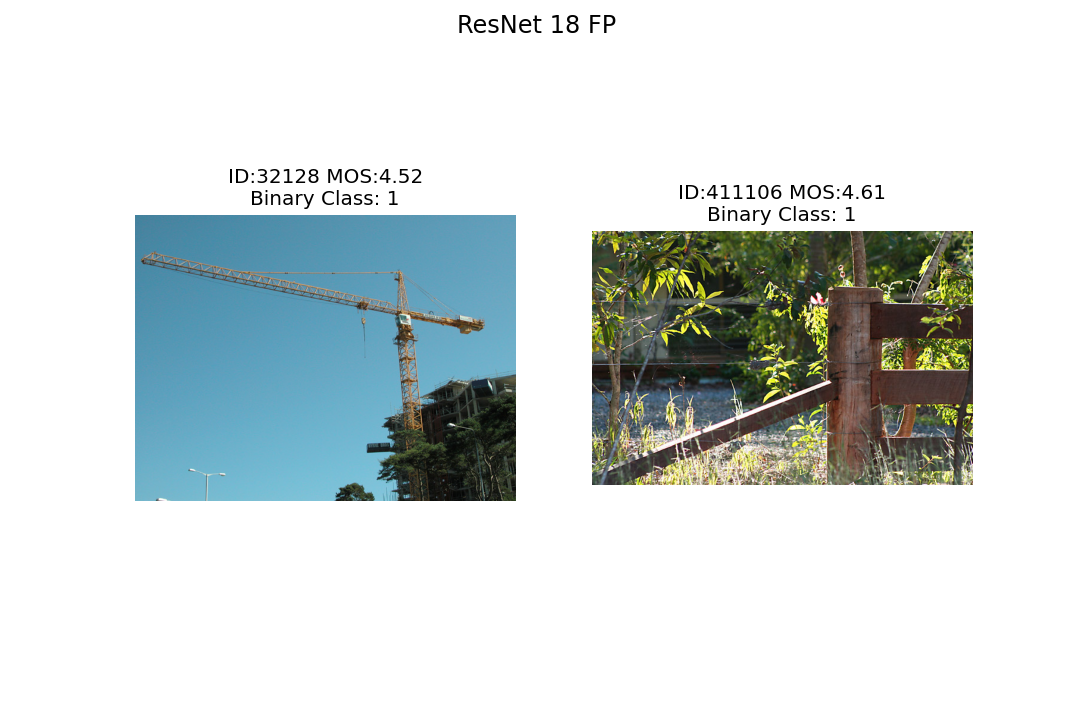
\includegraphics[width=0.333\textwidth]{figures/results_and_discussion/qualitative_results/false_positive/ResNet 18 FP .png}, \label{fig:ResNet_18_FP}}
    \caption{Examples of Exclusive False Positive Predictions by Each Network (Exclusive Set) on AVA Test Set}
    \label{fig:true_positive}
\end{figure}

ConViT $FP$ images appear to show a bias for global form, shown in figures (\ref{fig:ConViT_B_FP}, \ref{fig:ConViT_S_FP},\ref{fig:ConViT_Ti_FP}), however, not the MOS of figure \ref{fig:ConViT_Ti_FP}, which is exacly 5.0 where negative class is $\leq 5$. Figures (\ref{fig:ResNet_152_FP}, \ref{fig:ResNet_50_FP}, \ref{fig:ResNet_18_FP}) show $FPs$ exclusive to respective ResNets. 

\subsection{Training Metrics}

When shown in the same plot (figure \ref{fig:all models}), it is clear that ResNet50 and 152 overfit during training and that ConViTs (as well as CvT) consistently improve with accuracy in a more linear fashion. Further, it is noteworthy that ViT (pure transformer) shows a dip in initial training accuracy during training, and validation loss steadily increases.

\begin{figure}[ht]
    \centering
    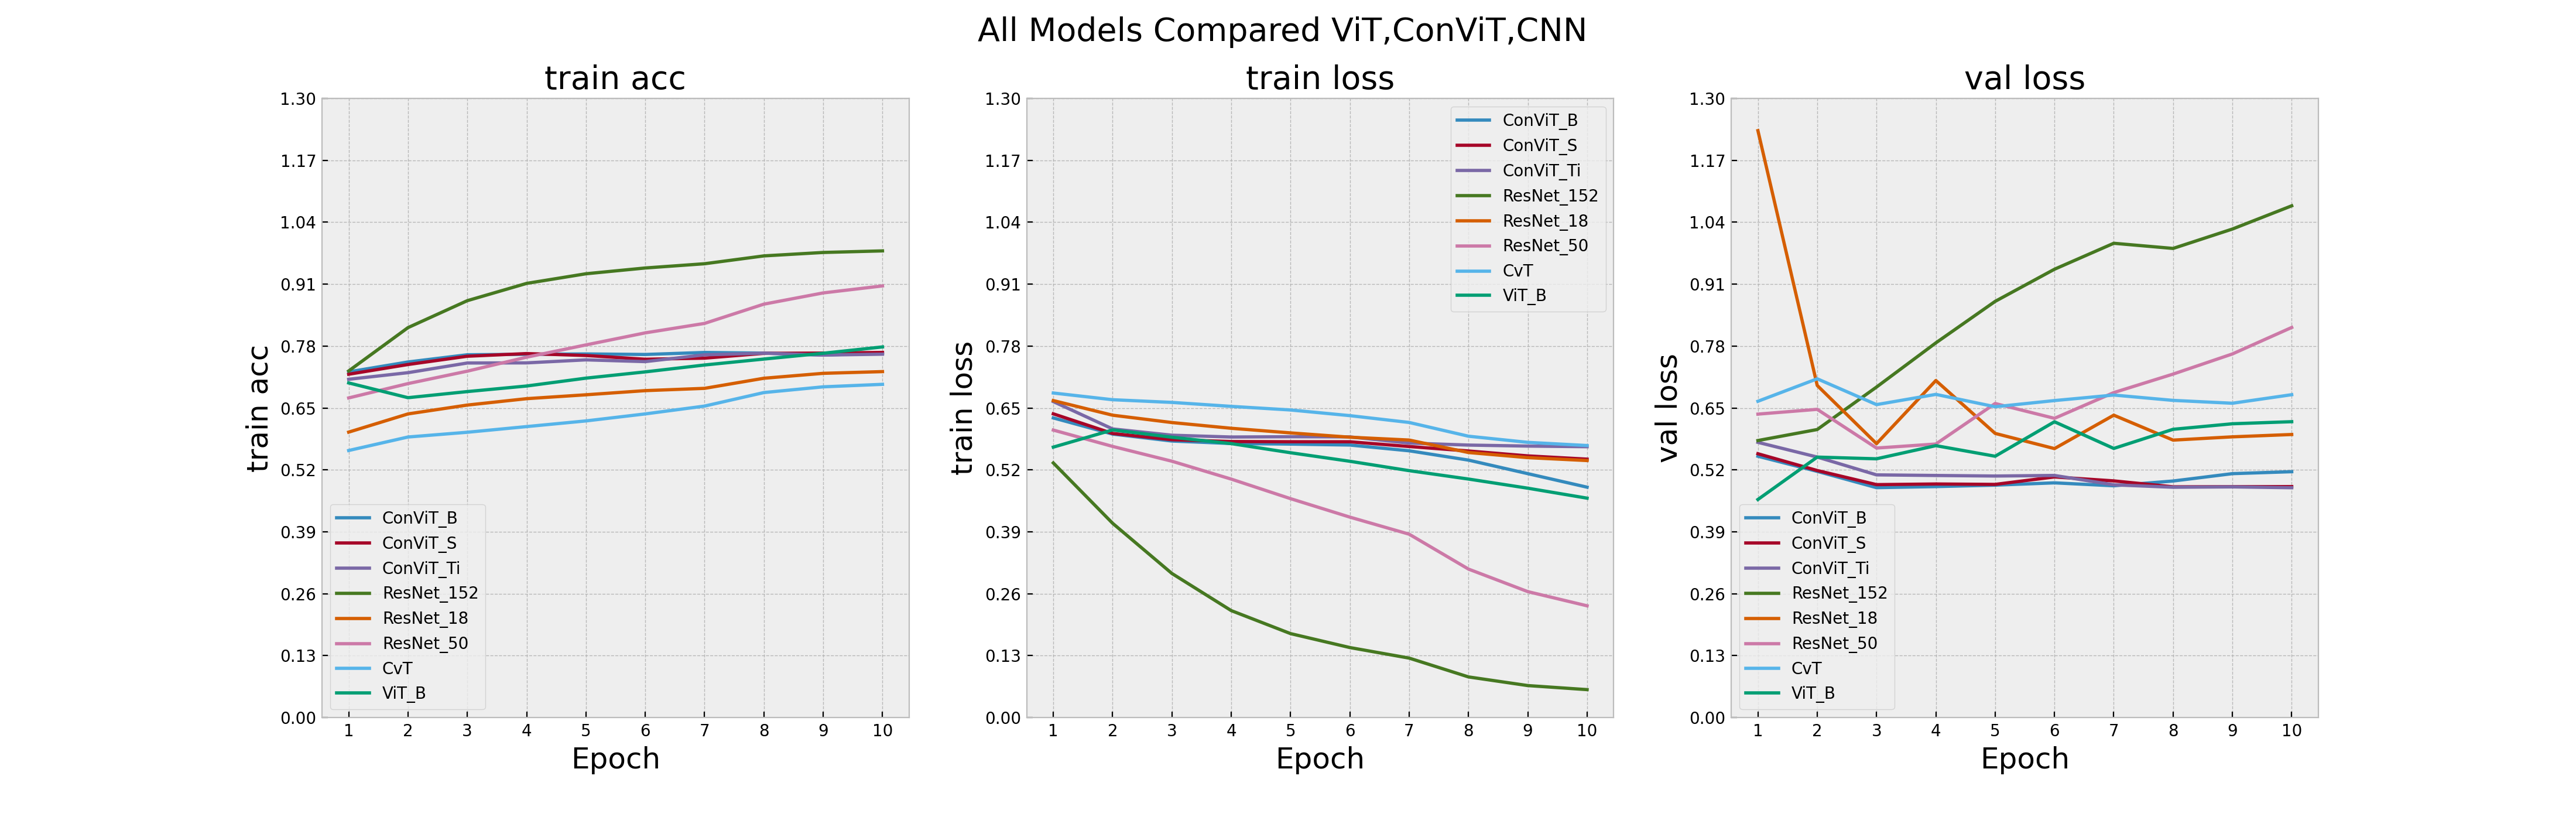
\includegraphics[width=0.99\textwidth]{figures/results_and_discussion/All Models Compared ViT,ConViT,CNN .png}
    \caption{All Models Compared}
    \label{fig:all models}
\end{figure}


High maximum validation loss for all of the ResNet models is shown in table \ref{tab:summary of training}. It is also noteworthy that ViT B performs well on the validation set (outstripping all other models which declined after first epoch).  
\begin{table}[ht!]
\small
    \centering
    \begin{tabular}{lrrrr}
\toprule
{} &  Train. Acc. &  Train. Loss &  Val. Acc. &  Val. Loss \\
\midrule
ViT B      &      0.778 &       0.604 &    0.786 &     0.621 \\
ConViT B   &      0.766 &       0.629 &    0.781 &     0.549 \\
ConViT S   &      0.767 &       0.638 &    0.746 &     0.554 \\
ConViT Ti  &      0.765 &       0.663 &    0.762 &     0.578 \\
ResNet 152 &      0.980 &       0.535 &    0.741 &     1.074 \\
ResNet 50  &      0.906 &       0.604 &    0.710 &     0.819 \\
ResNet 18  &      0.726 &       0.665 &    0.706 &     1.232 \\
CvT        &      0.700 &       0.681 &    0.625 &     0.711 \\

\bottomrule
\end{tabular}
\caption{Overall Maximum Training Results Compared}
    \label{tab:summary of training}
\end{table}

\newpage

We also show inference times and training times per epoch to give additional compute resources, and show how models might perform when embedded in a real world application (table \ref{tab:compute time}). ConVit B is clearly resource intensive. 



\begin{table}[ht!]
    \centering
    \tiny 
   \begin{tabular}{lccc}
\toprule
{} &  \# Million Trainable Params. & Train Time Per Epoch 230k Images & Inference Time 19k Images\\
\midrule
ResNet 18  &        11.2 & 56 mins.  & 3 mins.\\
ResNet 50  &        23.5 & 73 mins.  & 4 mins.\\
ResNet 152 &        58.1 & 121 mins. & 5 mins.\\
ConViT Ti  &         5.5 & 78 mins.  & 3 mins.\\
ConViT S   &        27.3 & 92 mins.  & 4 mins.\\
ConViT B   &        85.8 & 144 mins. & 5 mins.\\
ViT B      &        85.8 & 121 mins. & 5 mins.\\
CvT        &        17.6 & 94 mins.  & 4 mins.\\
\bottomrule
\end{tabular}
    \caption{Number Parameters and Training Time Per Epoch 230k Images on 1 GPU- batch size 10 Inference on 19k Images on AVA dataset}
    \label{tab:compute time}
\end{table}

